\chapter{High-Level and Low-Level Design}
\label{ch:design}

This chapter presents the design of the KhetLens software: the system as a whole, the considerations that shaped it, the architecture and its subsystems, the main design strategies and the alternatives we considered, the class structure of the mobile application, the sequence of interactions for the main use cases, and the policies we follow in implementation. The design realises the requirements of Chapter~\ref{ch:srs} and carries the diagnostic core of Chapter~\ref{ch:method} to the farmer's phone.

\section{System Overview}
KhetLens has four parts (Figure~\ref{fig:arch}). The \textbf{mobile application}, written in Kotlin, holds all farmer-facing functionality and is designed so that every use case works without a network: it captures and checks the photograph, runs the quantised model, applies the uncertainty check and the weather adjustment, drives the follow-up questions, looks up guidance in the local content pack, plays audio, and stores history and feedback locally. The \textbf{KhetLens server}, a small FastAPI service on PostgreSQL, has few responsibilities: one-time verification, feedback collection, distribution of model and content updates, and aggregate analytics. Two \textbf{external services} are used: a weather API, called by the phone when it is connected, and a WhatsApp-based one-time code service, called by the server. The \textbf{training pipeline} is an offline Python system that produces model releases; its outputs (model, class map, thresholds, novelty statistics) are consumed by the app.

The design approach can be summed up as \emph{offline-first, local-compute, data-as-content}. Everything a farmer needs is on the phone; the network is used opportunistically; and everything an agronomist might want to change (disease entries, guidance, questions, the weather table, audio) is data in a versioned content pack rather than code.

\section{Design Considerations}
The design is shaped by what the system may assume, the constraints it must respect, the principles we chose to follow, and our development method.

\subsection{Assumptions and Dependencies}
\begin{itemize}
  \item \textbf{Platform:} Android 8.1 or later on entry-level phones; CPU-only inference; camera and GPS present. The app depends on the standard Android libraries, the TensorFlow Lite runtime and Kotlin coroutines.
  \item \textbf{Model contract:} the app depends on a model release with a fixed interface: an image tensor in, and the backbone features, crop logits and per-crop disease logits out, with a manifest giving the class map, input size and thresholds. Any model that follows the contract can be swapped in.
  \item \textbf{Content contract:} the app depends on a content pack that follows a JSON schema (conditions, guidance, questions, weather table, audio list), validated at publish time.
  \item \textbf{Users:} farmers who may not read and use the phone one-handed outdoors; field officers who install and demonstrate the app; agronomists who review content offline.
  \item \textbf{Likely changes:} the disease list will be refined after agronomist review (handled by per-crop heads and the class map); the weather provider may change (handled by an interface); more crops may be added later (handled by the head structure and content schema).
\end{itemize}

\subsection{General Constraints}
\begin{itemize}
  \item \textbf{Memory and compute:} a few gigabytes of RAM shared with the system; inference must complete in about two seconds on an entry-level CPU (NFR-01).
  \item \textbf{Network:} absent or intermittent; no farmer action may wait on it; all network work is deferrable and safe to retry (NFR-03).
  \item \textbf{Storage:} total install under 150\,MB (NFR-02); photographs stored at reduced resolution; audio compressed; history kept for six months; feedback removed from the phone once uploaded.
  \item \textbf{Security and privacy:} tokens in encrypted storage; TLS everywhere; photographs and GPS never uploaded without opt-in (NFR-08).
  \item \textbf{Standards:} Android accessibility guidelines for tap targets and contrast; correct bidirectional layout for Urdu and Punjabi.
\end{itemize}

\subsection{Goals and Guidelines}
\begin{itemize}
  \item \textbf{Offline-first.} Design every feature as if the network did not exist, then add synchronisation.
  \item \textbf{Never block the farmer.} Background work runs in deferred jobs and never shows a spinner on a farmer-facing screen.
  \item \textbf{Honesty over coverage.} A ``not sure'' outcome is a correct output with its own screen and actions, not an error.
  \item \textbf{Data over code.} Anything an agronomist might change is content, validated and hot-swappable.
  \item \textbf{Measure on real phones.} Latency and memory claims come from entry-level devices, not emulators.
  \item \textbf{Keep the backend small.} The server does nothing the phone could do.
  \item \textbf{Separate ML from UI.} The ML layer exposes a plain Kotlin interface so the model and the app can be developed and tested independently.
\end{itemize}

\subsection{Development Methods}
We follow an Agile process with two-week sprints, a backlog in GitHub Issues, pull requests reviewed by a second team member and automated checks on each change. Each sprint ends with a demonstration to our supervisor. Training runs are tracked with their configuration, data version and seeds so that results can be regenerated. The app follows the layered architecture common in Android (presentation, domain, data) with the ML components as a separate module, and the MVVM pattern in the presentation layer. We considered Flutter for the app and chose native Android because the inference runtime, camera control and Nastaliq text rendering are all first-class there and the project is Android-only by scope.

\section{System Architecture}
Figure~\ref{fig:arch} shows the high-level architecture. The dashed boundary around the phone marks the offline-capable region: every arrow inside it works without a network, and every arrow crossing it is marked ``when connected''.

\begin{figure}[H]
  \centering
  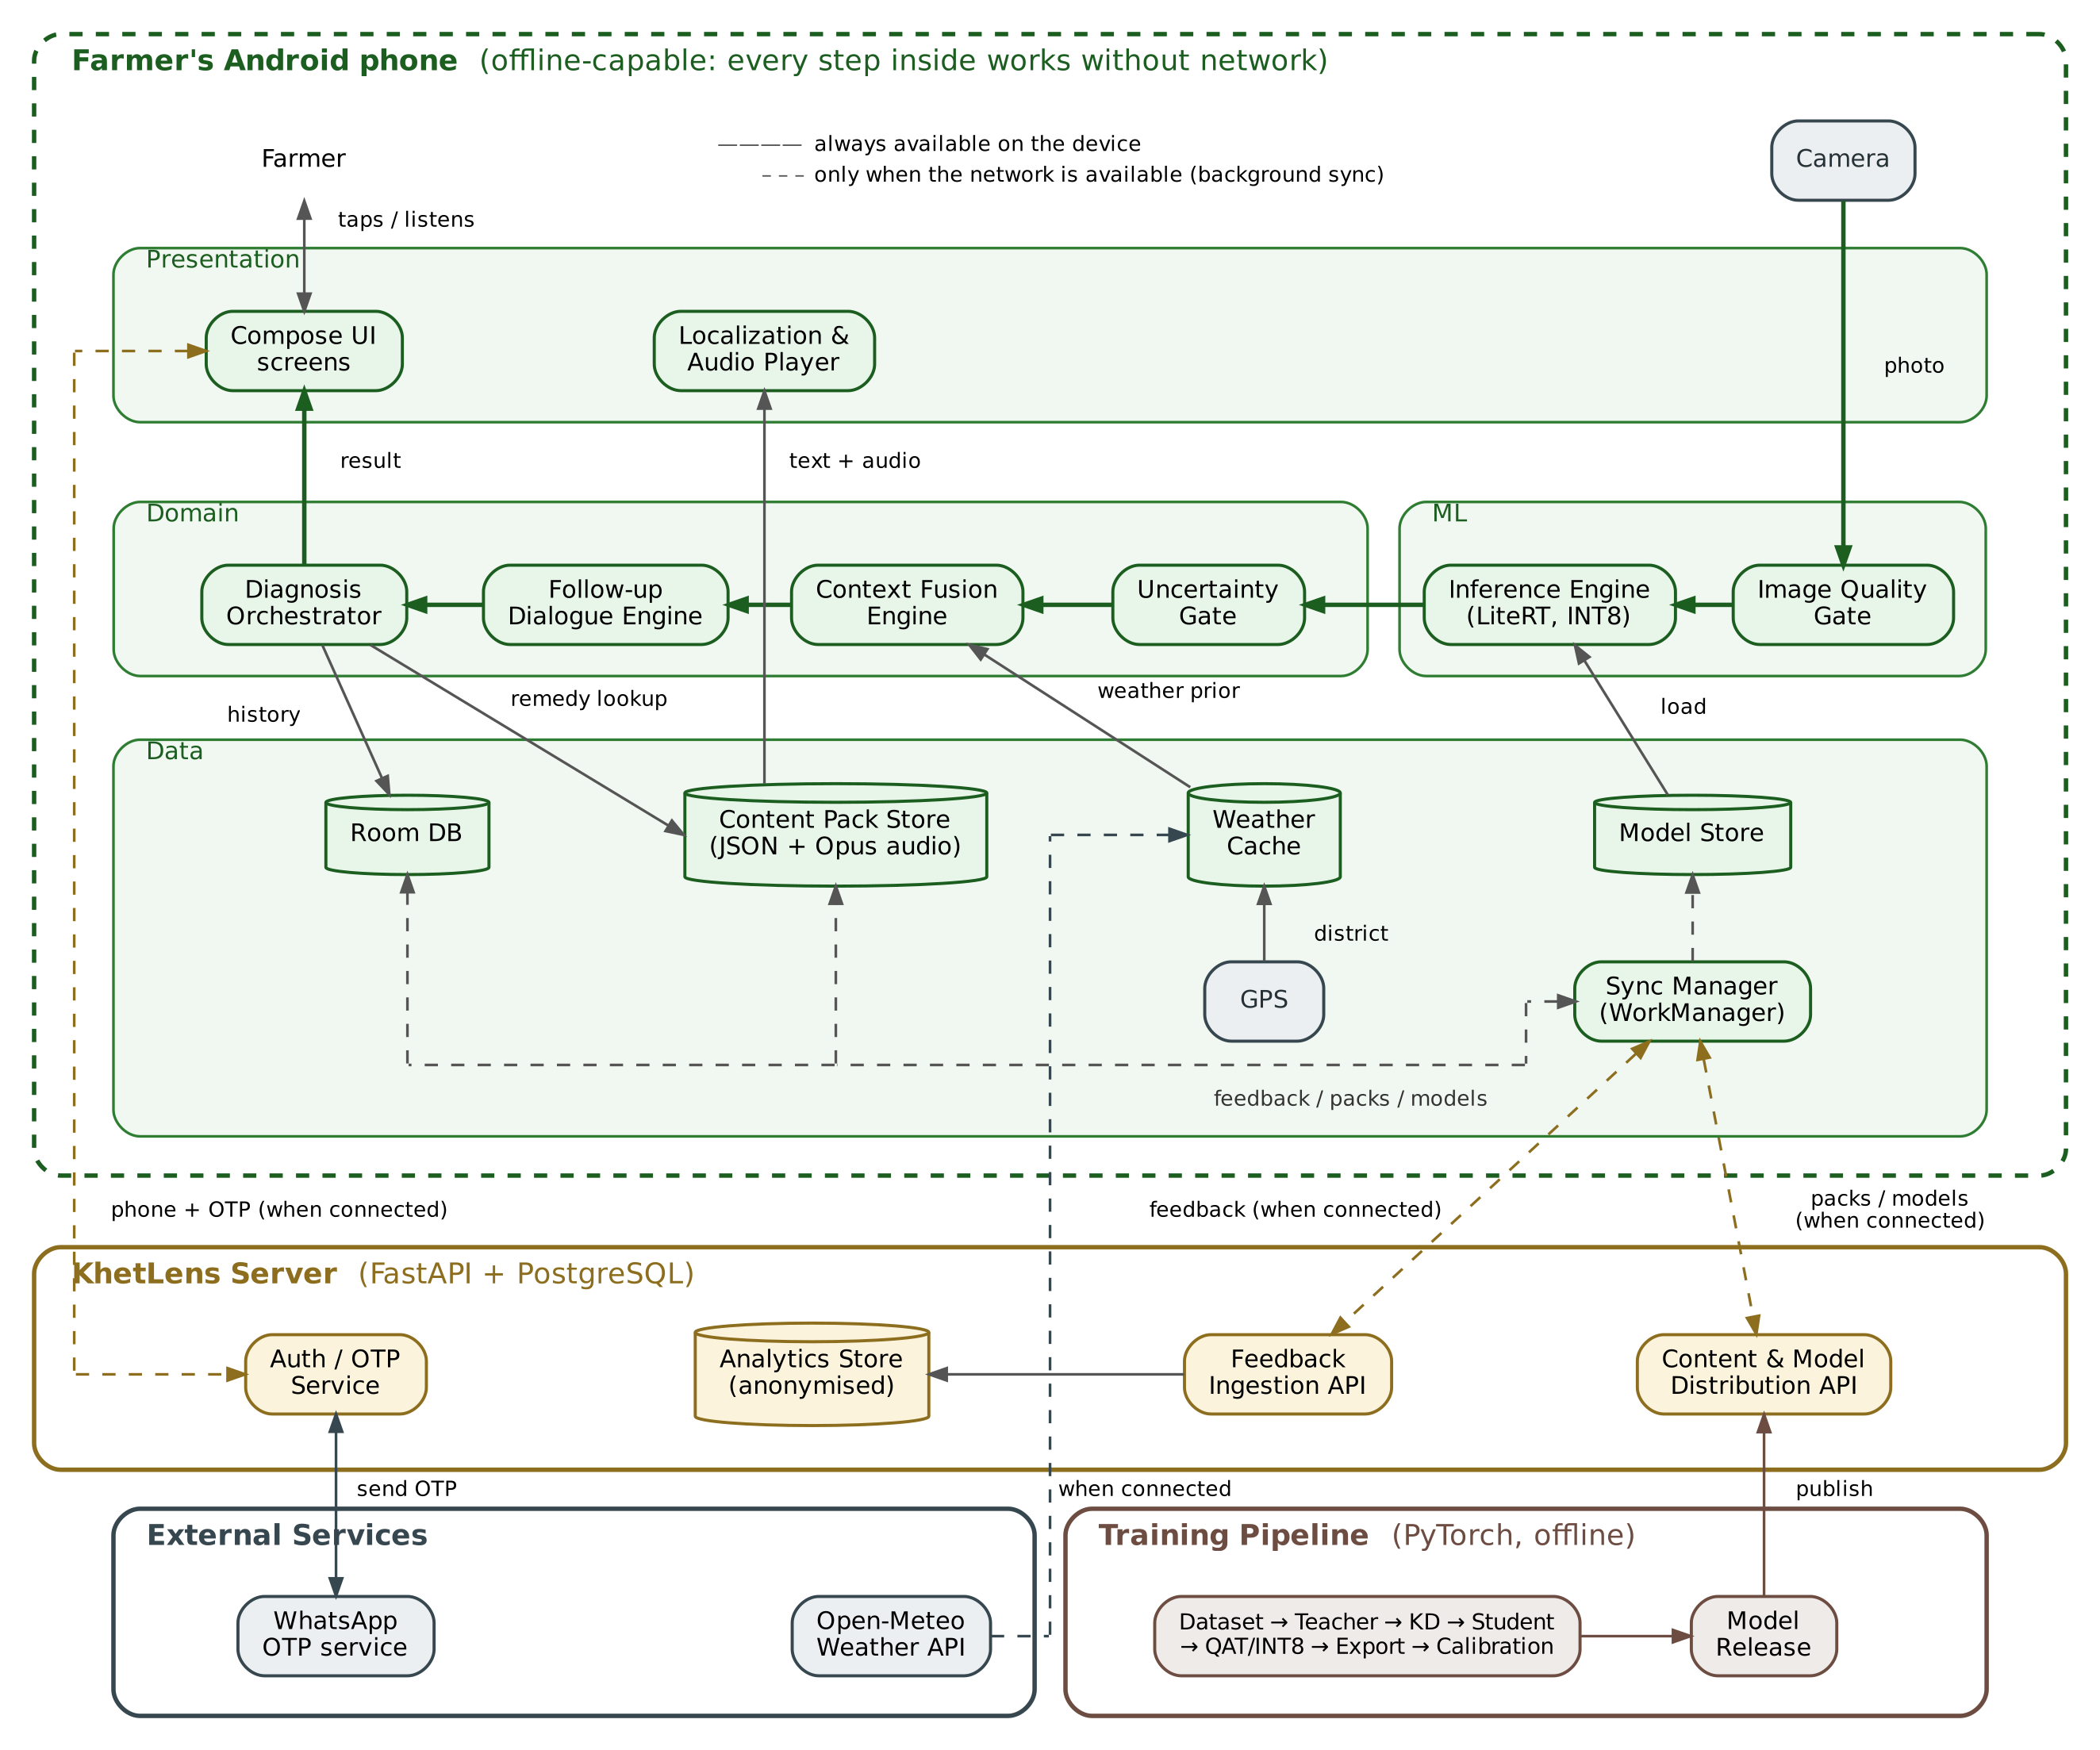
\includegraphics[width=\textwidth,height=0.88\textheight,keepaspectratio]{Figures/diagrams/architecture.png}
  \caption{High-level architecture of KhetLens. The mobile application (top) is fully functional offline; the server (middle) handles verification, feedback, distribution and analytics; the external services are the weather API and the WhatsApp code service; the offline training pipeline publishes model releases.}
  \label{fig:arch}
\end{figure}

The mobile application has four layers. The \emph{presentation} layer holds the screens, view models, localisation and audio player. The \emph{domain} layer holds the diagnostic logic independent of UI and storage: the diagnosis orchestrator (which runs Algorithm~\ref{algo:gate}), the weather adjustment and the follow-up engine. The \emph{ML} layer wraps the model: the image quality check, the inference engine and the uncertainty check. The \emph{data} layer holds persistence and I/O: the local database, the content pack store, the weather cache, the model store and the sync manager. Dependencies point inwards, so the diagnostic logic can be tested on a desktop against recorded inputs. We chose this decomposition because it separates the three things that change for different reasons: the interface (farmer feedback), the diagnostic logic (research results) and the platform code. A decomposition by feature was considered and set aside because the diagnostic core is shared by several features.

\subsection{Subsystem Architecture}
\textbf{Diagnosis subsystem.} Figure~\ref{fig:sub-diag} details the component every photograph passes through. The quality check computes the sharpness and exposure measures. The inference engine owns the interpreter, created once at start-up and reused; it runs the model on the whole photograph and, for wider shots, on its regions, and combines the outputs (Section~\ref{sec:multiscale}). The uncertainty check holds the release's statistics in memory. The weather adjustment reads the table from the content pack and the latest snapshot from the cache. The follow-up engine holds the question set and performs the update after each answer. The three outcomes are modelled as a sealed type so that every screen must handle every case.

\begin{figure}[H]
  \centering
  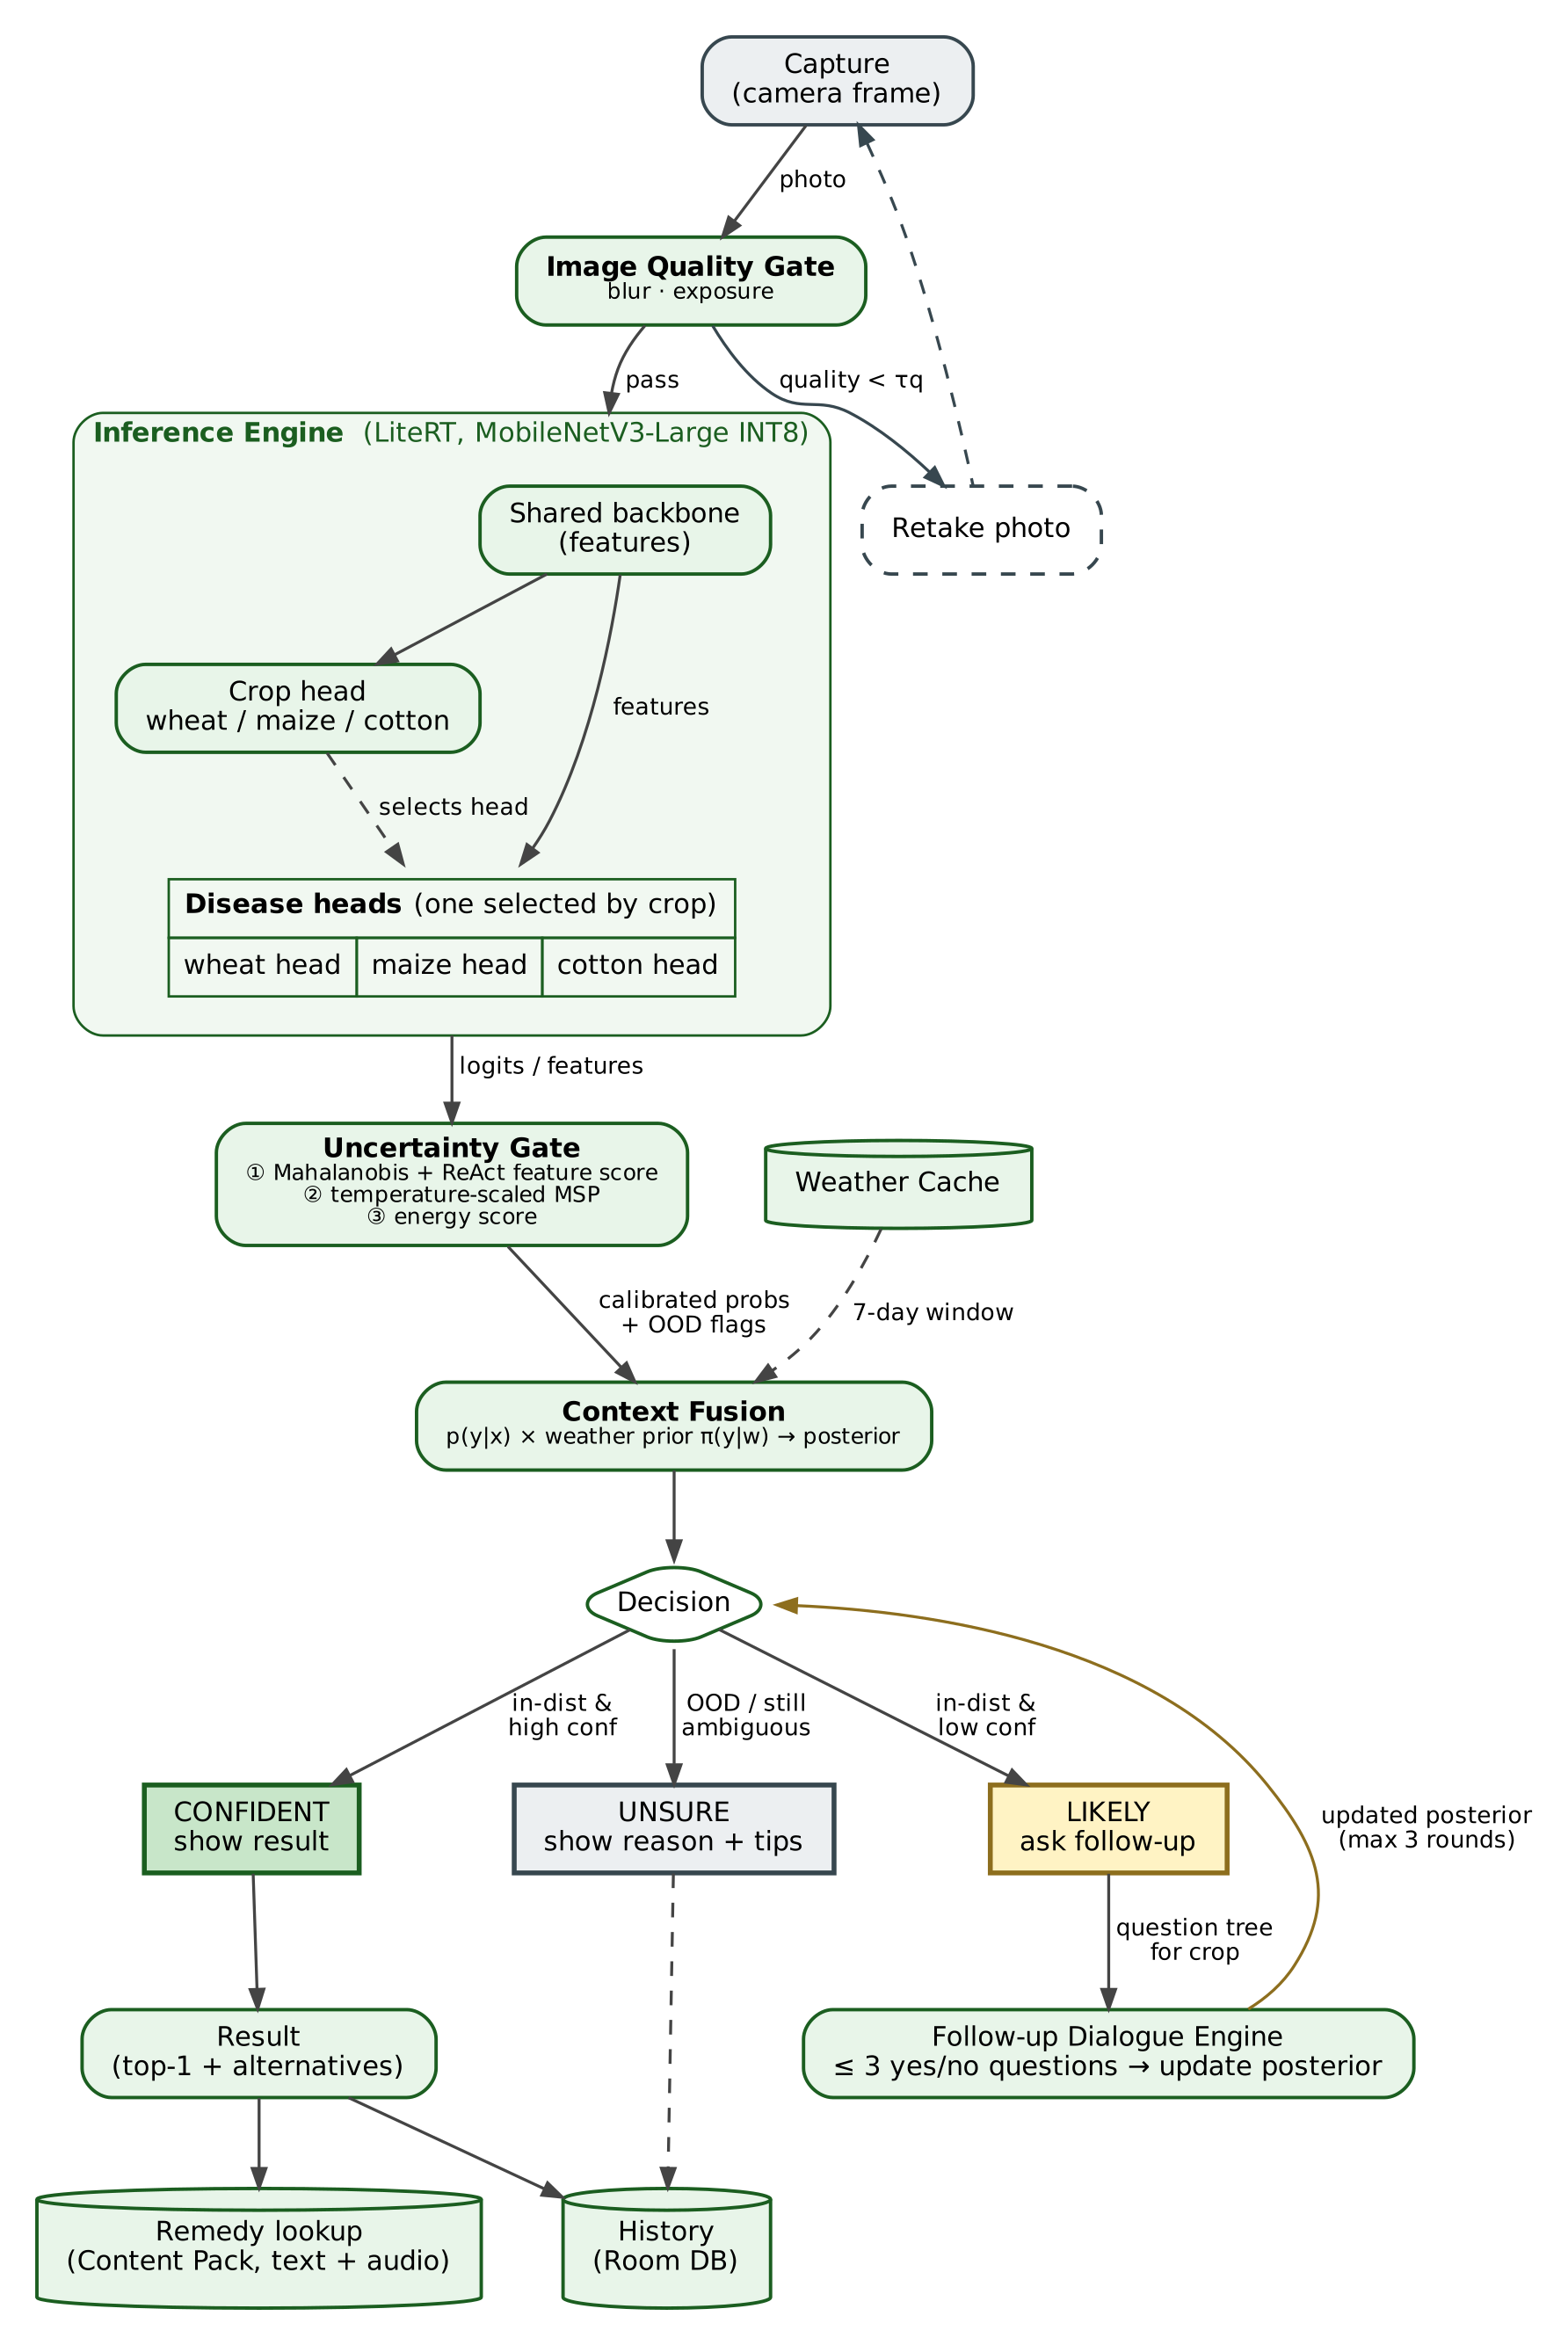
\includegraphics[width=\textwidth,height=0.88\textheight,keepaspectratio]{Figures/diagrams/subsystem_diagnosis.png}
  \caption{Component diagram of the diagnosis subsystem, from capture through the quality check, inference, uncertainty check and weather adjustment to the three outcomes, guidance lookup and history.}
  \label{fig:sub-diag}
\end{figure}

\textbf{Backend subsystem.} Figure~\ref{fig:sub-backend} shows the server. The FastAPI application has four routers. \emph{Auth} requests and verifies one-time codes through the WhatsApp service, limits requests per number, and returns a signed token; it stores only a hash of the number. \emph{Feedback} accepts batches of feedback records, deduplicates them by client-generated identifier so that retries are safe, and writes them to the database; opted-in images go to object storage. \emph{Distribution} serves version information and download links for content packs and model releases. \emph{Analytics} serves aggregate counts per district, crop and condition to the team. Our publish tool validates and uploads packs and releases after agronomist review.

\begin{figure}[H]
  \centering
  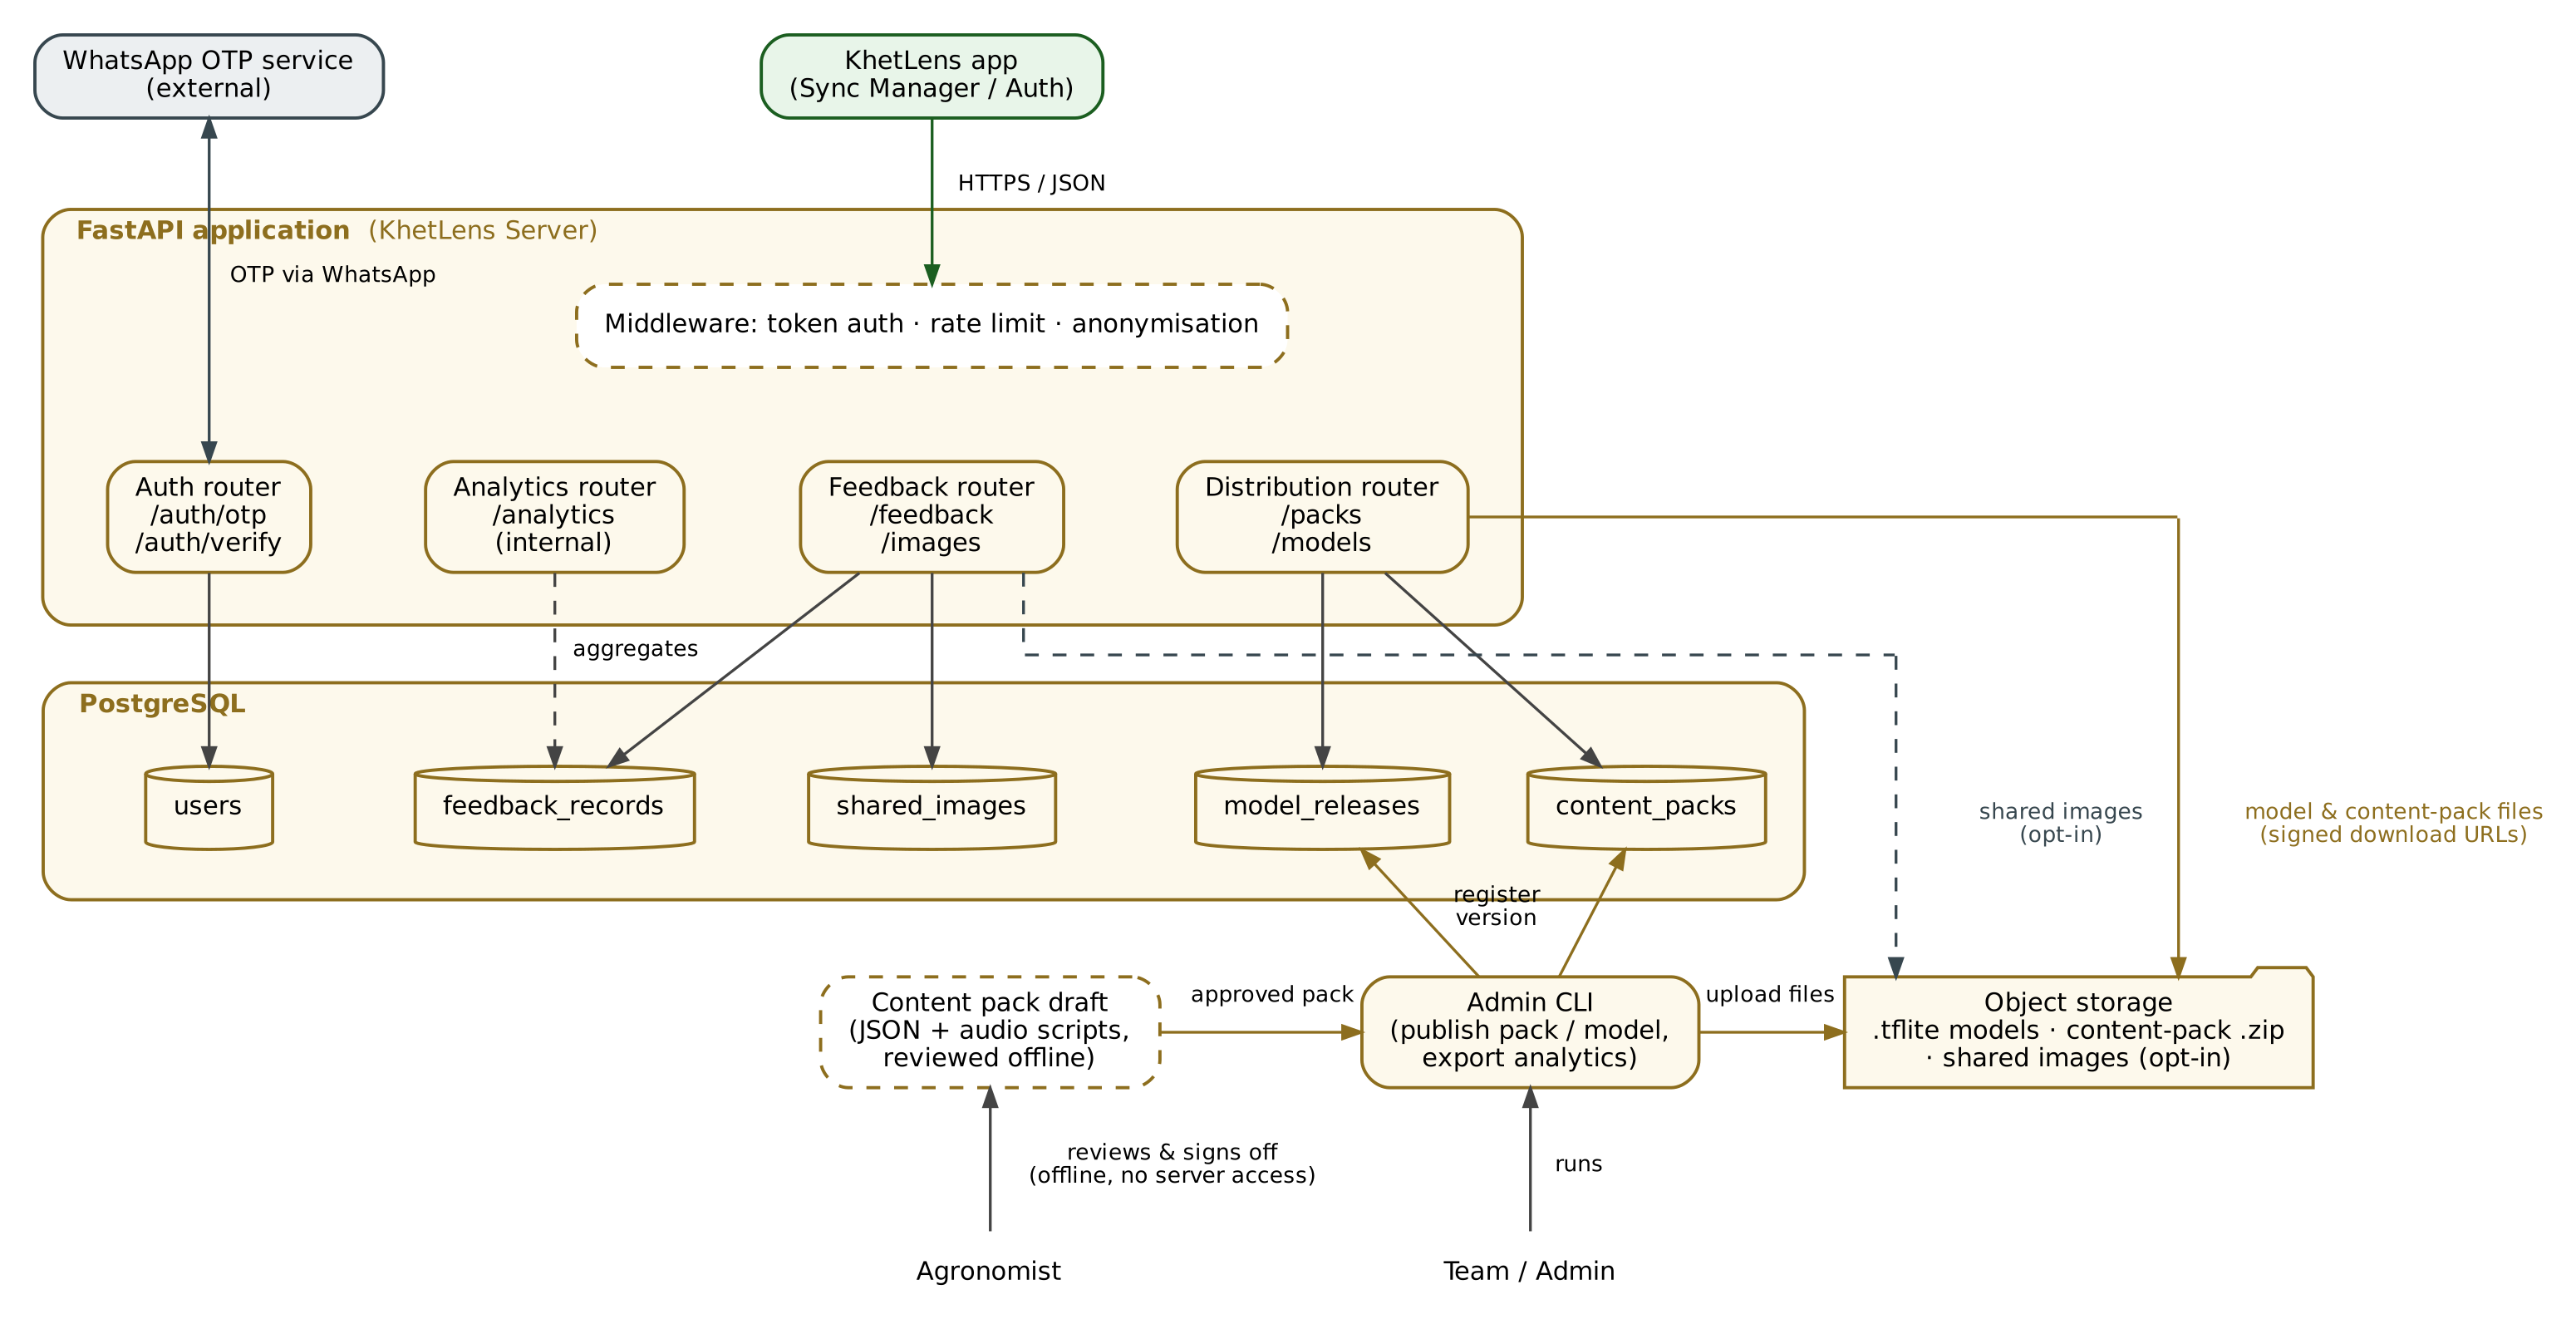
\includegraphics[width=\textwidth,height=0.88\textheight,keepaspectratio]{Figures/diagrams/subsystem_backend.png}
  \caption{Component diagram of the KhetLens server: routers, database tables, object storage, our publish tool and the agronomist review that precedes publication.}
  \label{fig:sub-backend}
\end{figure}

\section{Architectural Strategies}
Each strategy records the decision, the alternatives considered and the reasons.

\subsection{Local-compute, offline-first inference}
\textbf{Decision:} the full diagnosis runs on the device; there is no cloud inference path. \textbf{Alternatives:} cloud inference, or a hybrid with cloud fallback. \textbf{Reasons:} connectivity is the defining constraint of the problem; compact models have been run on entry-level phones in the field~\cite{ramcharan2019cassava} and quantised MobileNetV3 models are small and fast~\cite{khan2023edge}; privacy follows by construction; a single code path is easier to test.

\subsection{Native Android application}
\textbf{Decision:} Kotlin with Jetpack Compose. \textbf{Alternatives:} Flutter, React Native. \textbf{Reasons:} first-class support for the inference runtime, camera and local database; small install size; reliable right-to-left and Nastaliq rendering; Android-only scope.

\subsection{Quantised model with a measured runtime choice}
\textbf{Decision:} 8-bit integer model on TensorFlow Lite, with ONNX Runtime benchmarked as an alternative. \textbf{Alternatives:} 16-bit floats; other mobile runtimes. \textbf{Reasons:} integer models are smaller and faster on CPUs, and runtime choice has a large effect on latency~\cite{zhangq2022mobilebench}, so we measure rather than assume.

\subsection{Shared backbone with crop and per-crop disease heads}
\textbf{Decision:} one network with a crop head and three disease heads. \textbf{Alternatives:} three separate models, or one flat 17-way classifier. \textbf{Reasons:} crop-conditional design improved field accuracy in prior work~\cite{picon2019cropcond}; classes can be added to one head without retraining the backbone; the crop head gives a natural confirmation step.

\subsection{Rule-based weather adjustment}
\textbf{Decision:} multiply calibrated probabilities by a prior from a reviewed table (Equation~\ref{eq:fusion}). \textbf{Alternatives:} learned fusion of weather features inside the network. \textbf{Reasons:} transparency to agronomists and farmers (the Why panel can state the weather cue), no need for paired training data, editability without retraining, and graceful fallback when weather is unavailable.

\subsection{Data as content in versioned packs}
\textbf{Decision:} disease entries, guidance, questions, the weather table and audio form a validated, versioned content pack downloaded and swapped atomically. \textbf{Alternatives:} content compiled into the app; a server-rendered content API. \textbf{Reasons:} agronomist corrections should not need an app release; the pack is also the unit of review and attribution.

\subsection{Opportunistic, retry-safe synchronisation}
\textbf{Decision:} all network work runs in deferred background jobs with network constraints, back-off and client-generated identifiers. \textbf{Alternatives:} synchronous calls at the moment of action. \textbf{Reasons:} the farmer is never blocked, and retries cannot create duplicates.

\subsection{Privacy by default}
\textbf{Decision:} photographs and GPS coordinates stay on the device; the server receives district, crop, outcome, confidence and versions; sharing a photograph is a per-feedback opt-in. \textbf{Reasons:} NFR-08 and the trust that farmer adoption depends on~\cite{soodan2024adoption}.

\subsection{Error detection and recovery}
Every external interaction has a defined failure behaviour: a failed quality check returns to the viewfinder with a reason; a model that fails to load falls back to the last working one, ultimately the baseline bundled in the app (FR-26); a corrupt or partial download is discarded; stale weather yields a uniform prior and a visible note; a failed sign-in offers retry and guest mode; database writes are transactional so an interrupted diagnosis leaves no partial record.

\subsection{Concurrency and memory}
Inference runs on a dedicated single-threaded dispatcher so that two diagnoses never contend for the interpreter; live preview analysis runs on a separate dispatcher with frame dropping. Images are decoded at the model's input size directly from the camera buffer; history photographs are stored downscaled and removed with their records after six months.

\section{Domain Model/Class Diagram}
Figure~\ref{fig:class} shows the domain model of the mobile application. The persistent entities map onto the tables of Section~\ref{sec:db}: \texttt{User}, \texttt{Diagnosis}, \texttt{WeatherSnapshot}, \texttt{Remedy} and \texttt{Feedback} to the tables of the same name, \texttt{Disease} to \texttt{condition}, and \texttt{ContentPack} to \texttt{content\_pack\_version}; \texttt{ModelRelease} is the manifest of the installed model. The services carry behaviour: \texttt{DiagnosisOrchestrator} implements Algorithm~\ref{algo:gate} by composing \texttt{InferenceEngine}, \texttt{UncertaintyGate}, \texttt{ContextFusionEngine} and \texttt{FollowUpEngine}; \texttt{WeatherRepository} and \texttt{ContentRepository} are interfaces implemented in the data layer; \texttt{SyncManager} schedules the background jobs.

\begin{figure}[H]
  \centering
  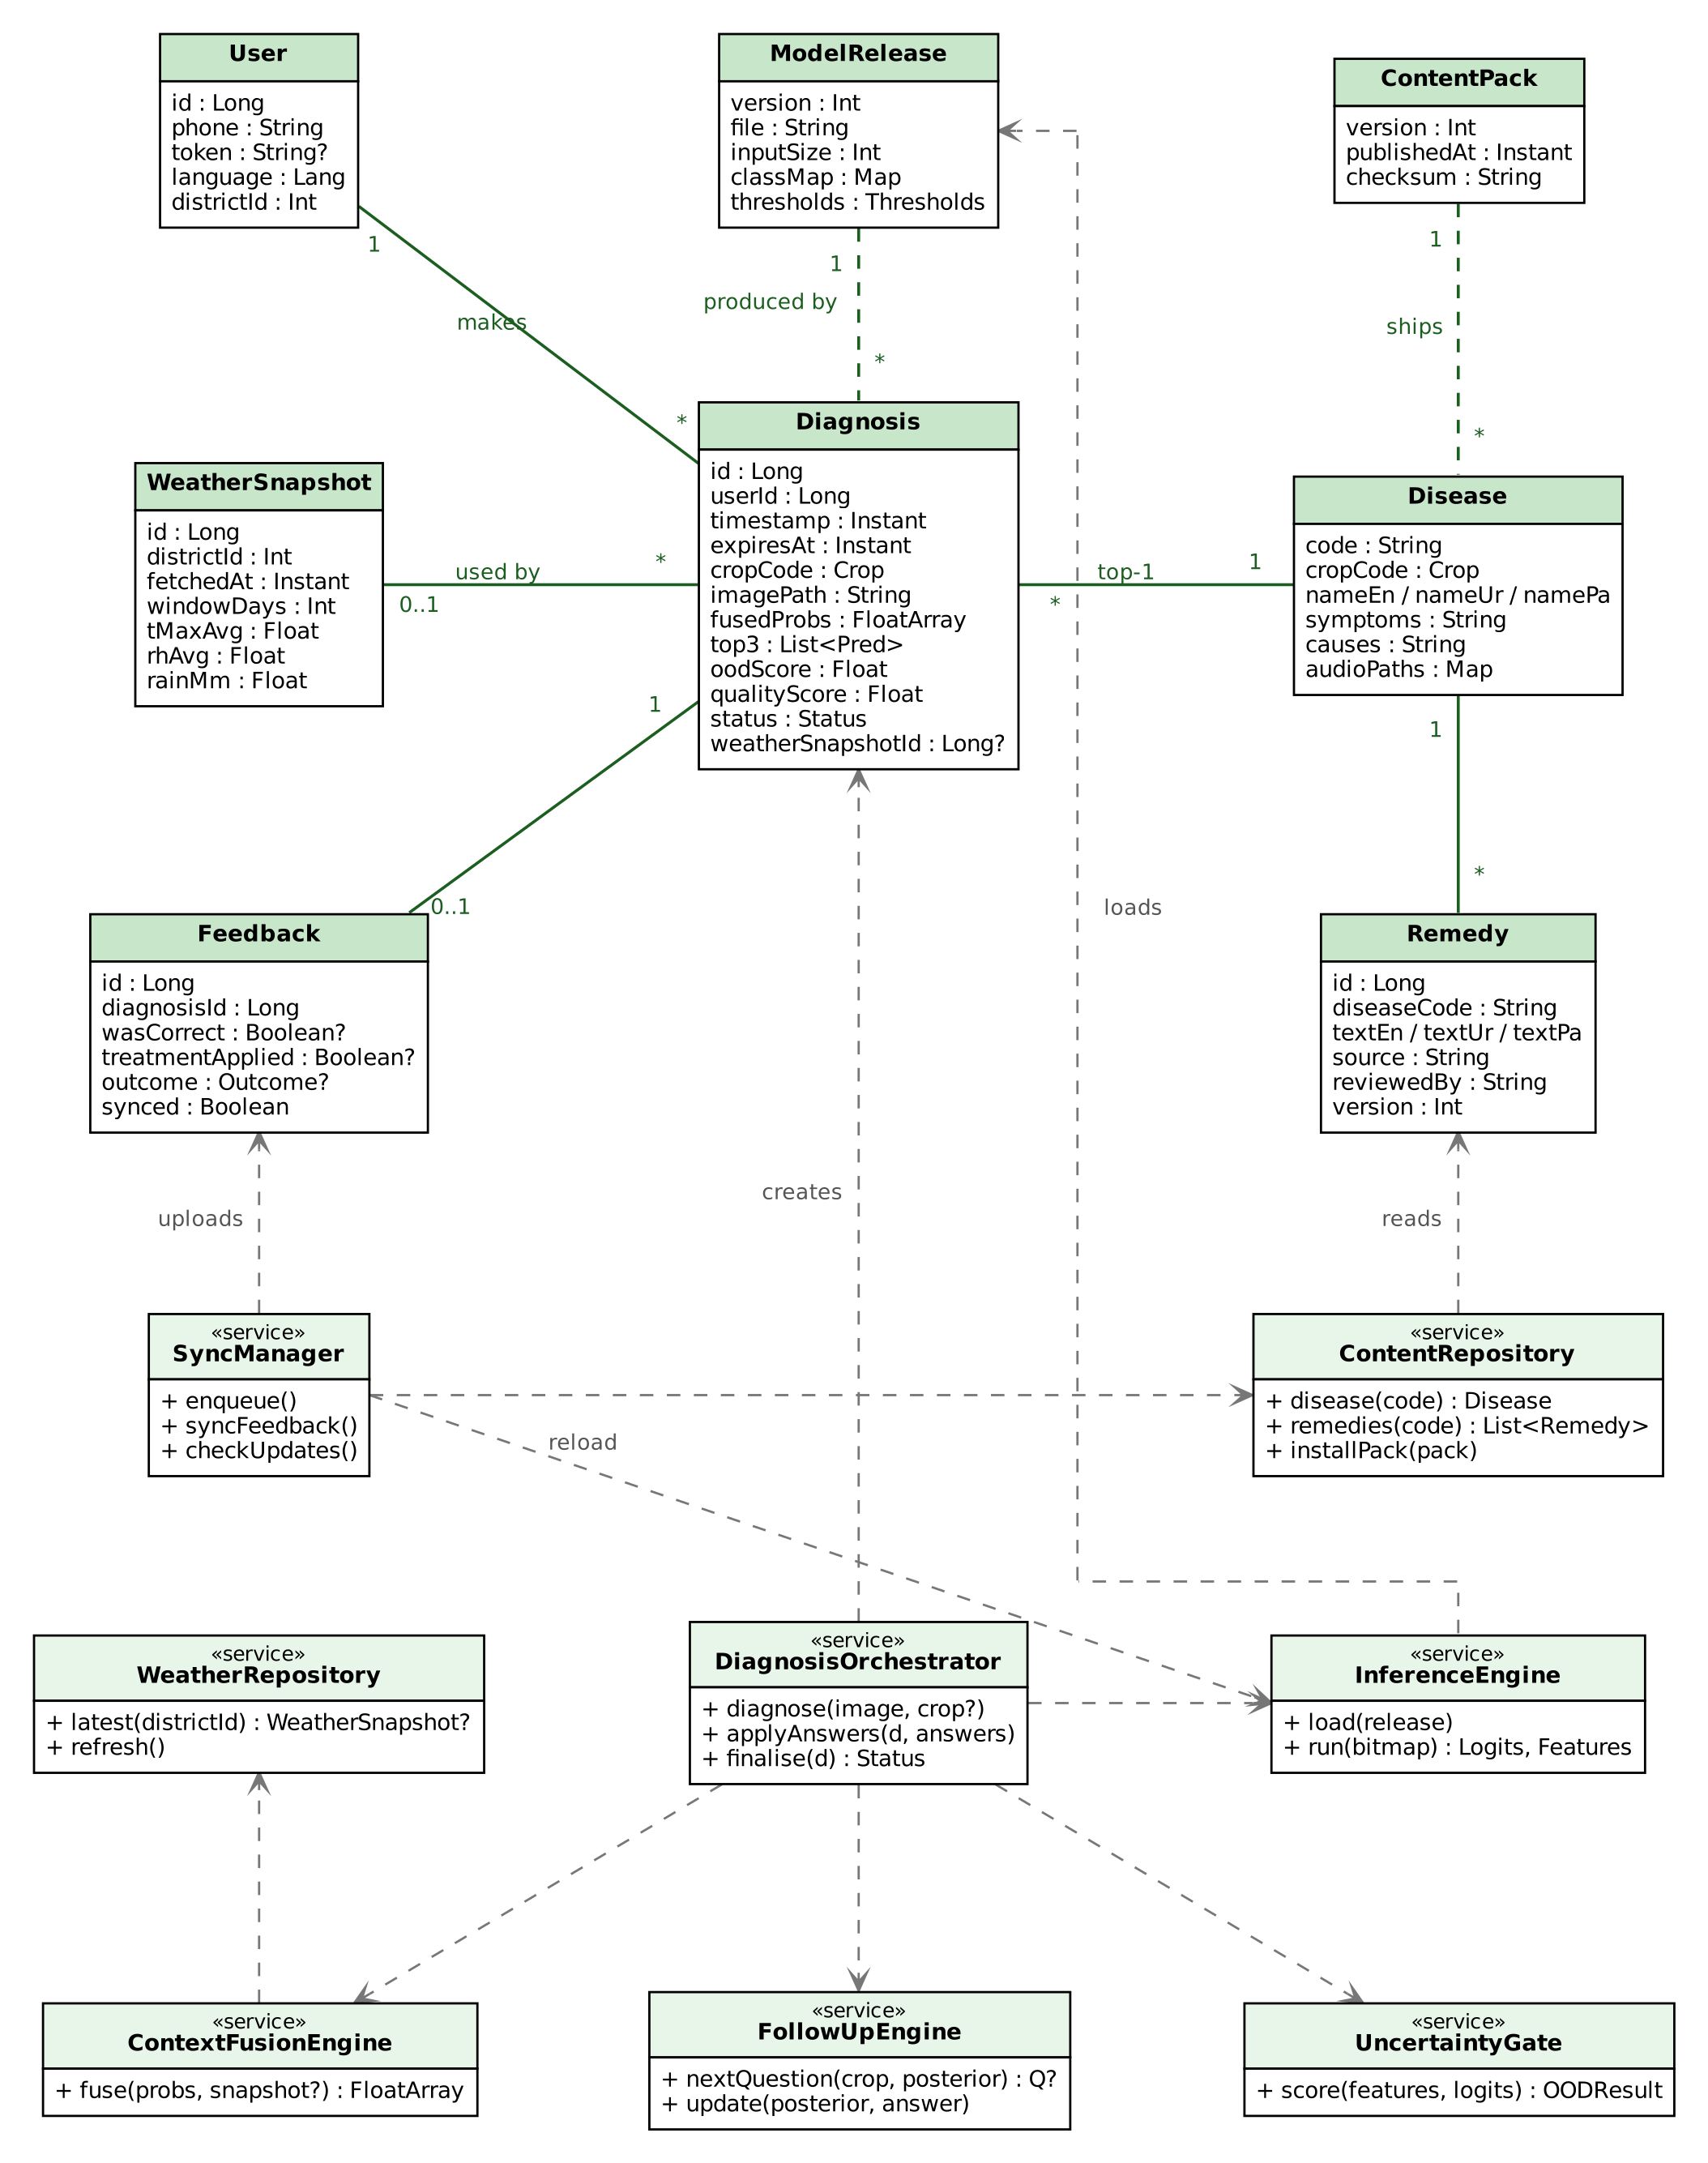
\includegraphics[width=\textwidth,height=0.88\textheight,keepaspectratio]{Figures/diagrams/class_diagram.png}
  \caption{Class diagram of the mobile application: persistent entities with their key attributes and relationships, and the domain and data services that operate on them.}
  \label{fig:class}
\end{figure}

\section{Sequence Diagrams}
Five interactions define the system's behaviour; each is traced to its use case.

\textbf{Diagnose a plant (UC-04, UC-05).} Figure~\ref{fig:seq-diag} shows the main path and the quality-check rejection. The shutter tap hands the frame to the diagnosis engine, which checks quality, runs the model, applies the uncertainty check and the weather adjustment, stores the record and returns the outcome to the screen.

\begin{figure}[H]
  \centering
  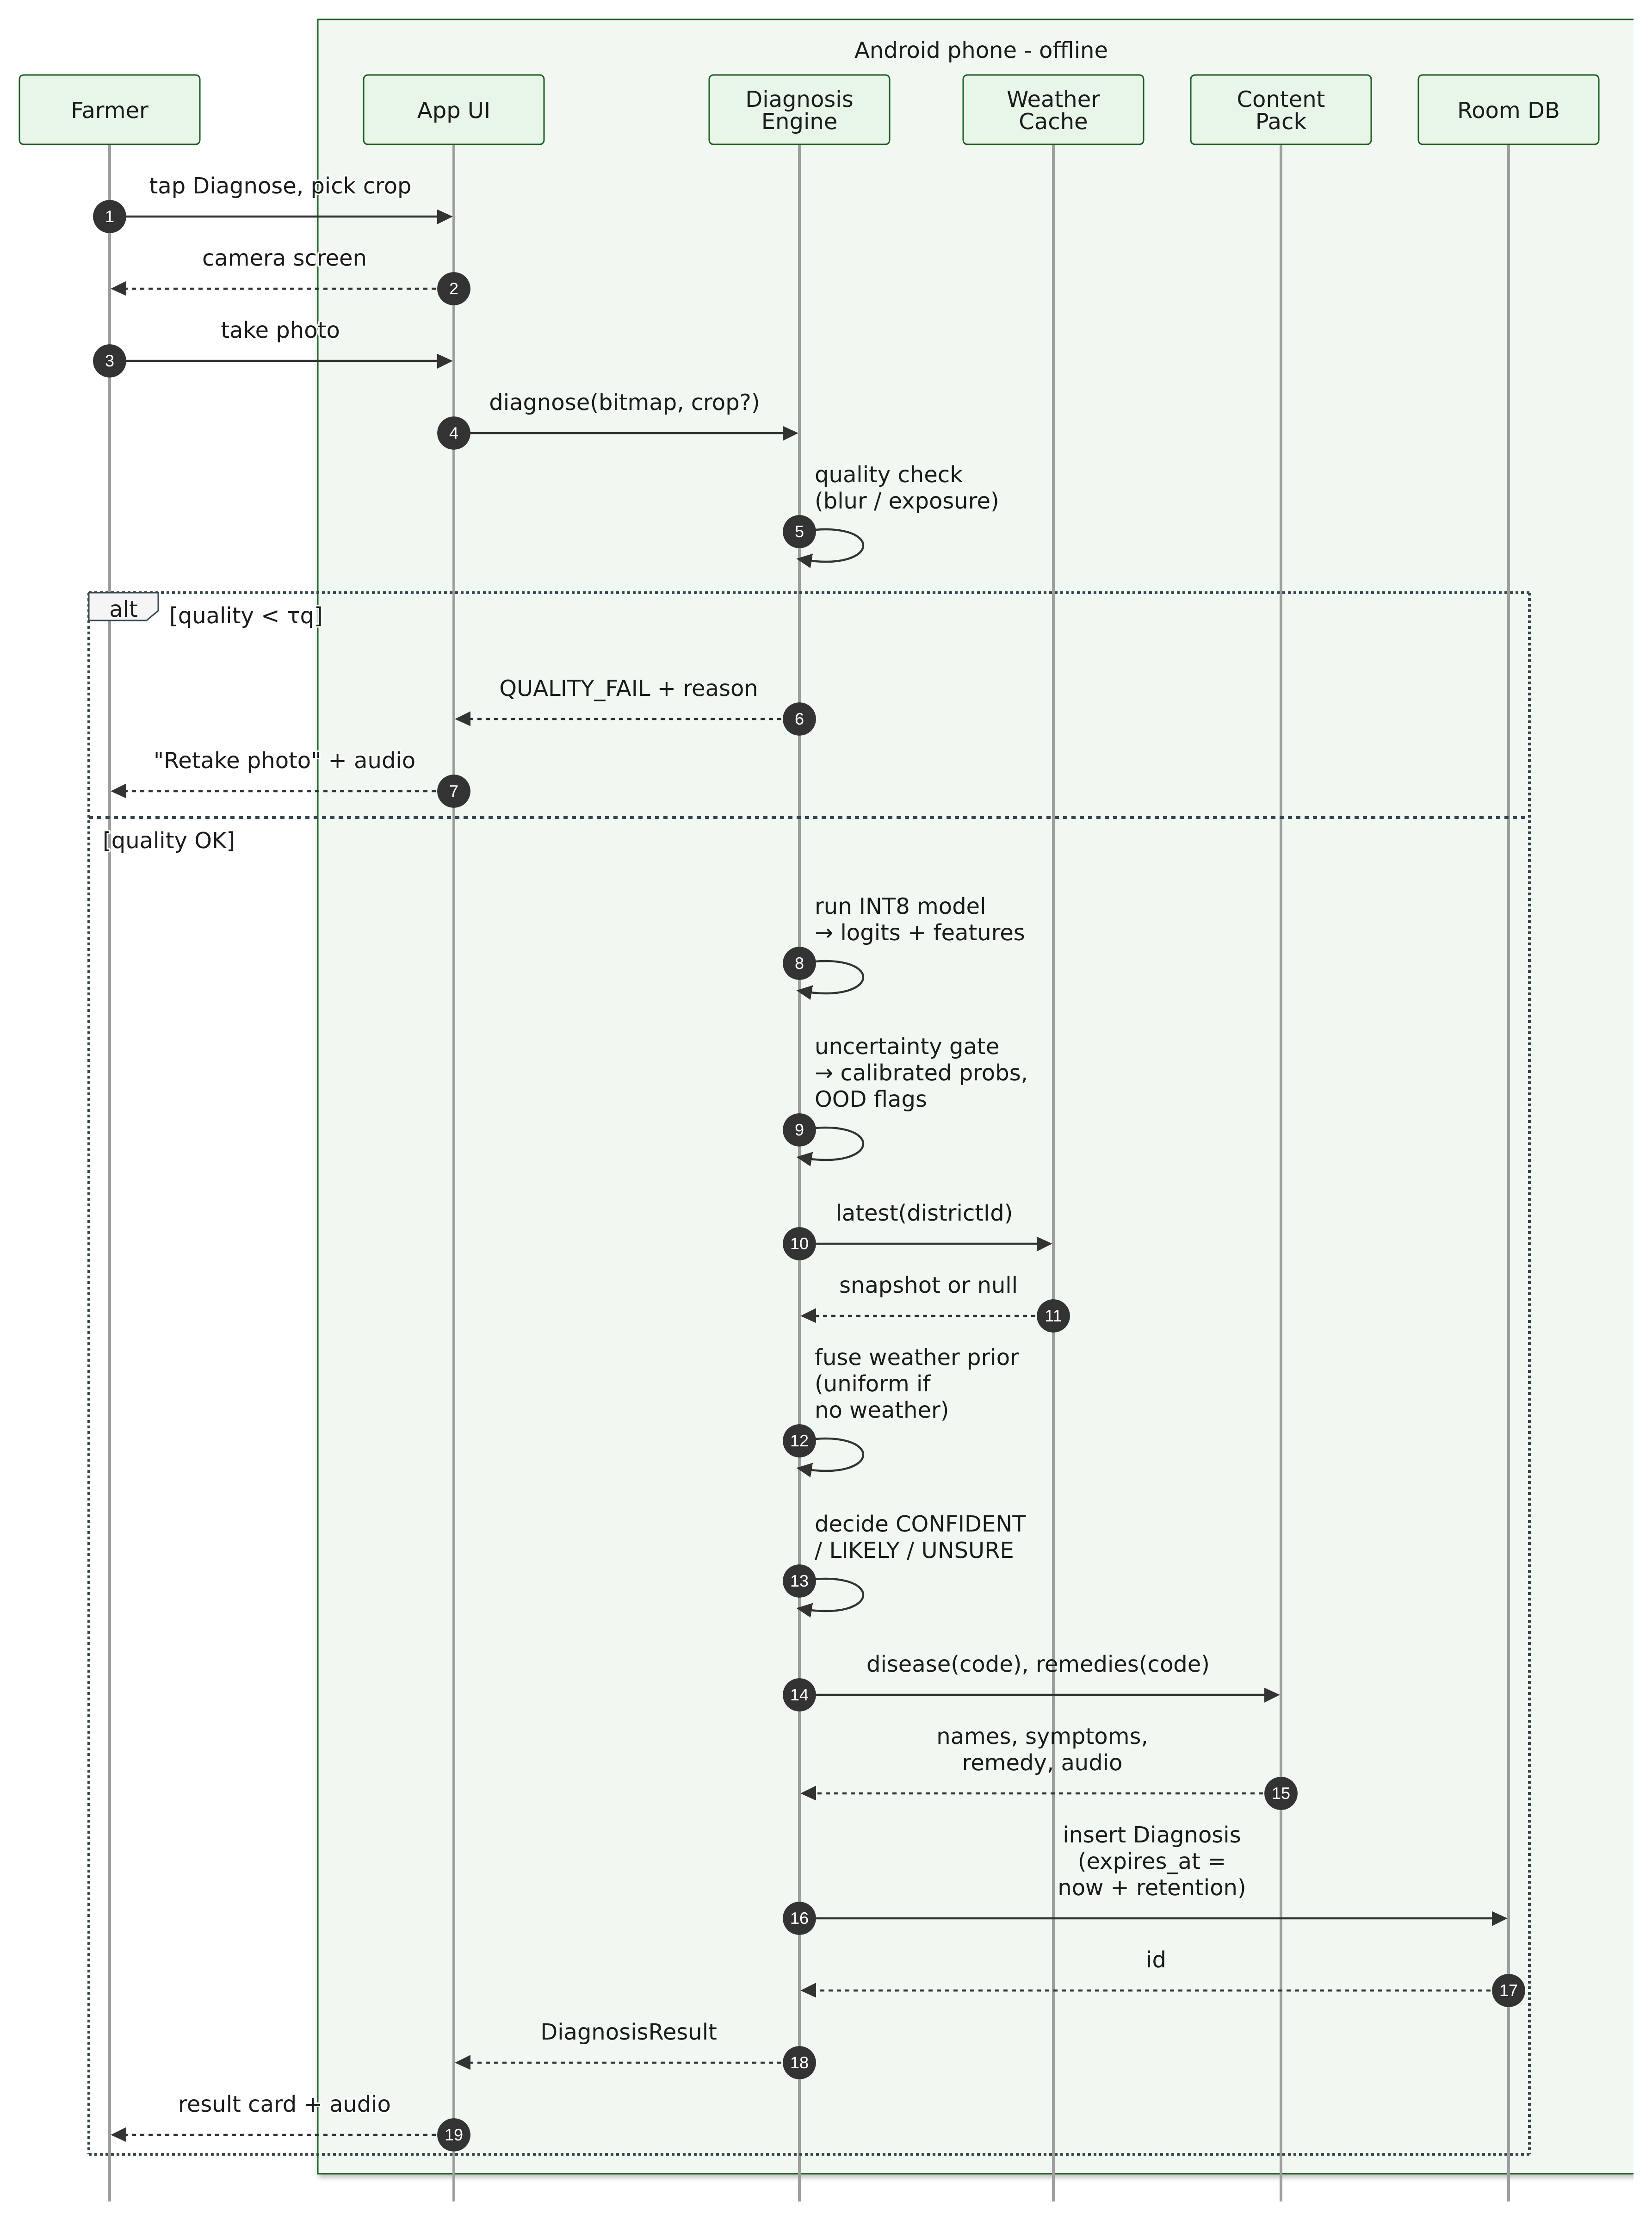
\includegraphics[width=\textwidth,height=0.88\textheight,keepaspectratio]{Figures/diagrams/seq_diagnose.png}
  \caption{Sequence diagram for a diagnosis, including the alternative flow in which the quality check rejects the photograph.}
  \label{fig:seq-diag}
\end{figure}

\textbf{Follow-up questions (UC-07).} Figure~\ref{fig:seq-follow} shows the Likely branch: the follow-up engine loads the crop's question set, the screen asks up to three questions, each answer updates the result, and the orchestrator finalises and stores the answers.

\begin{figure}[H]
  \centering
  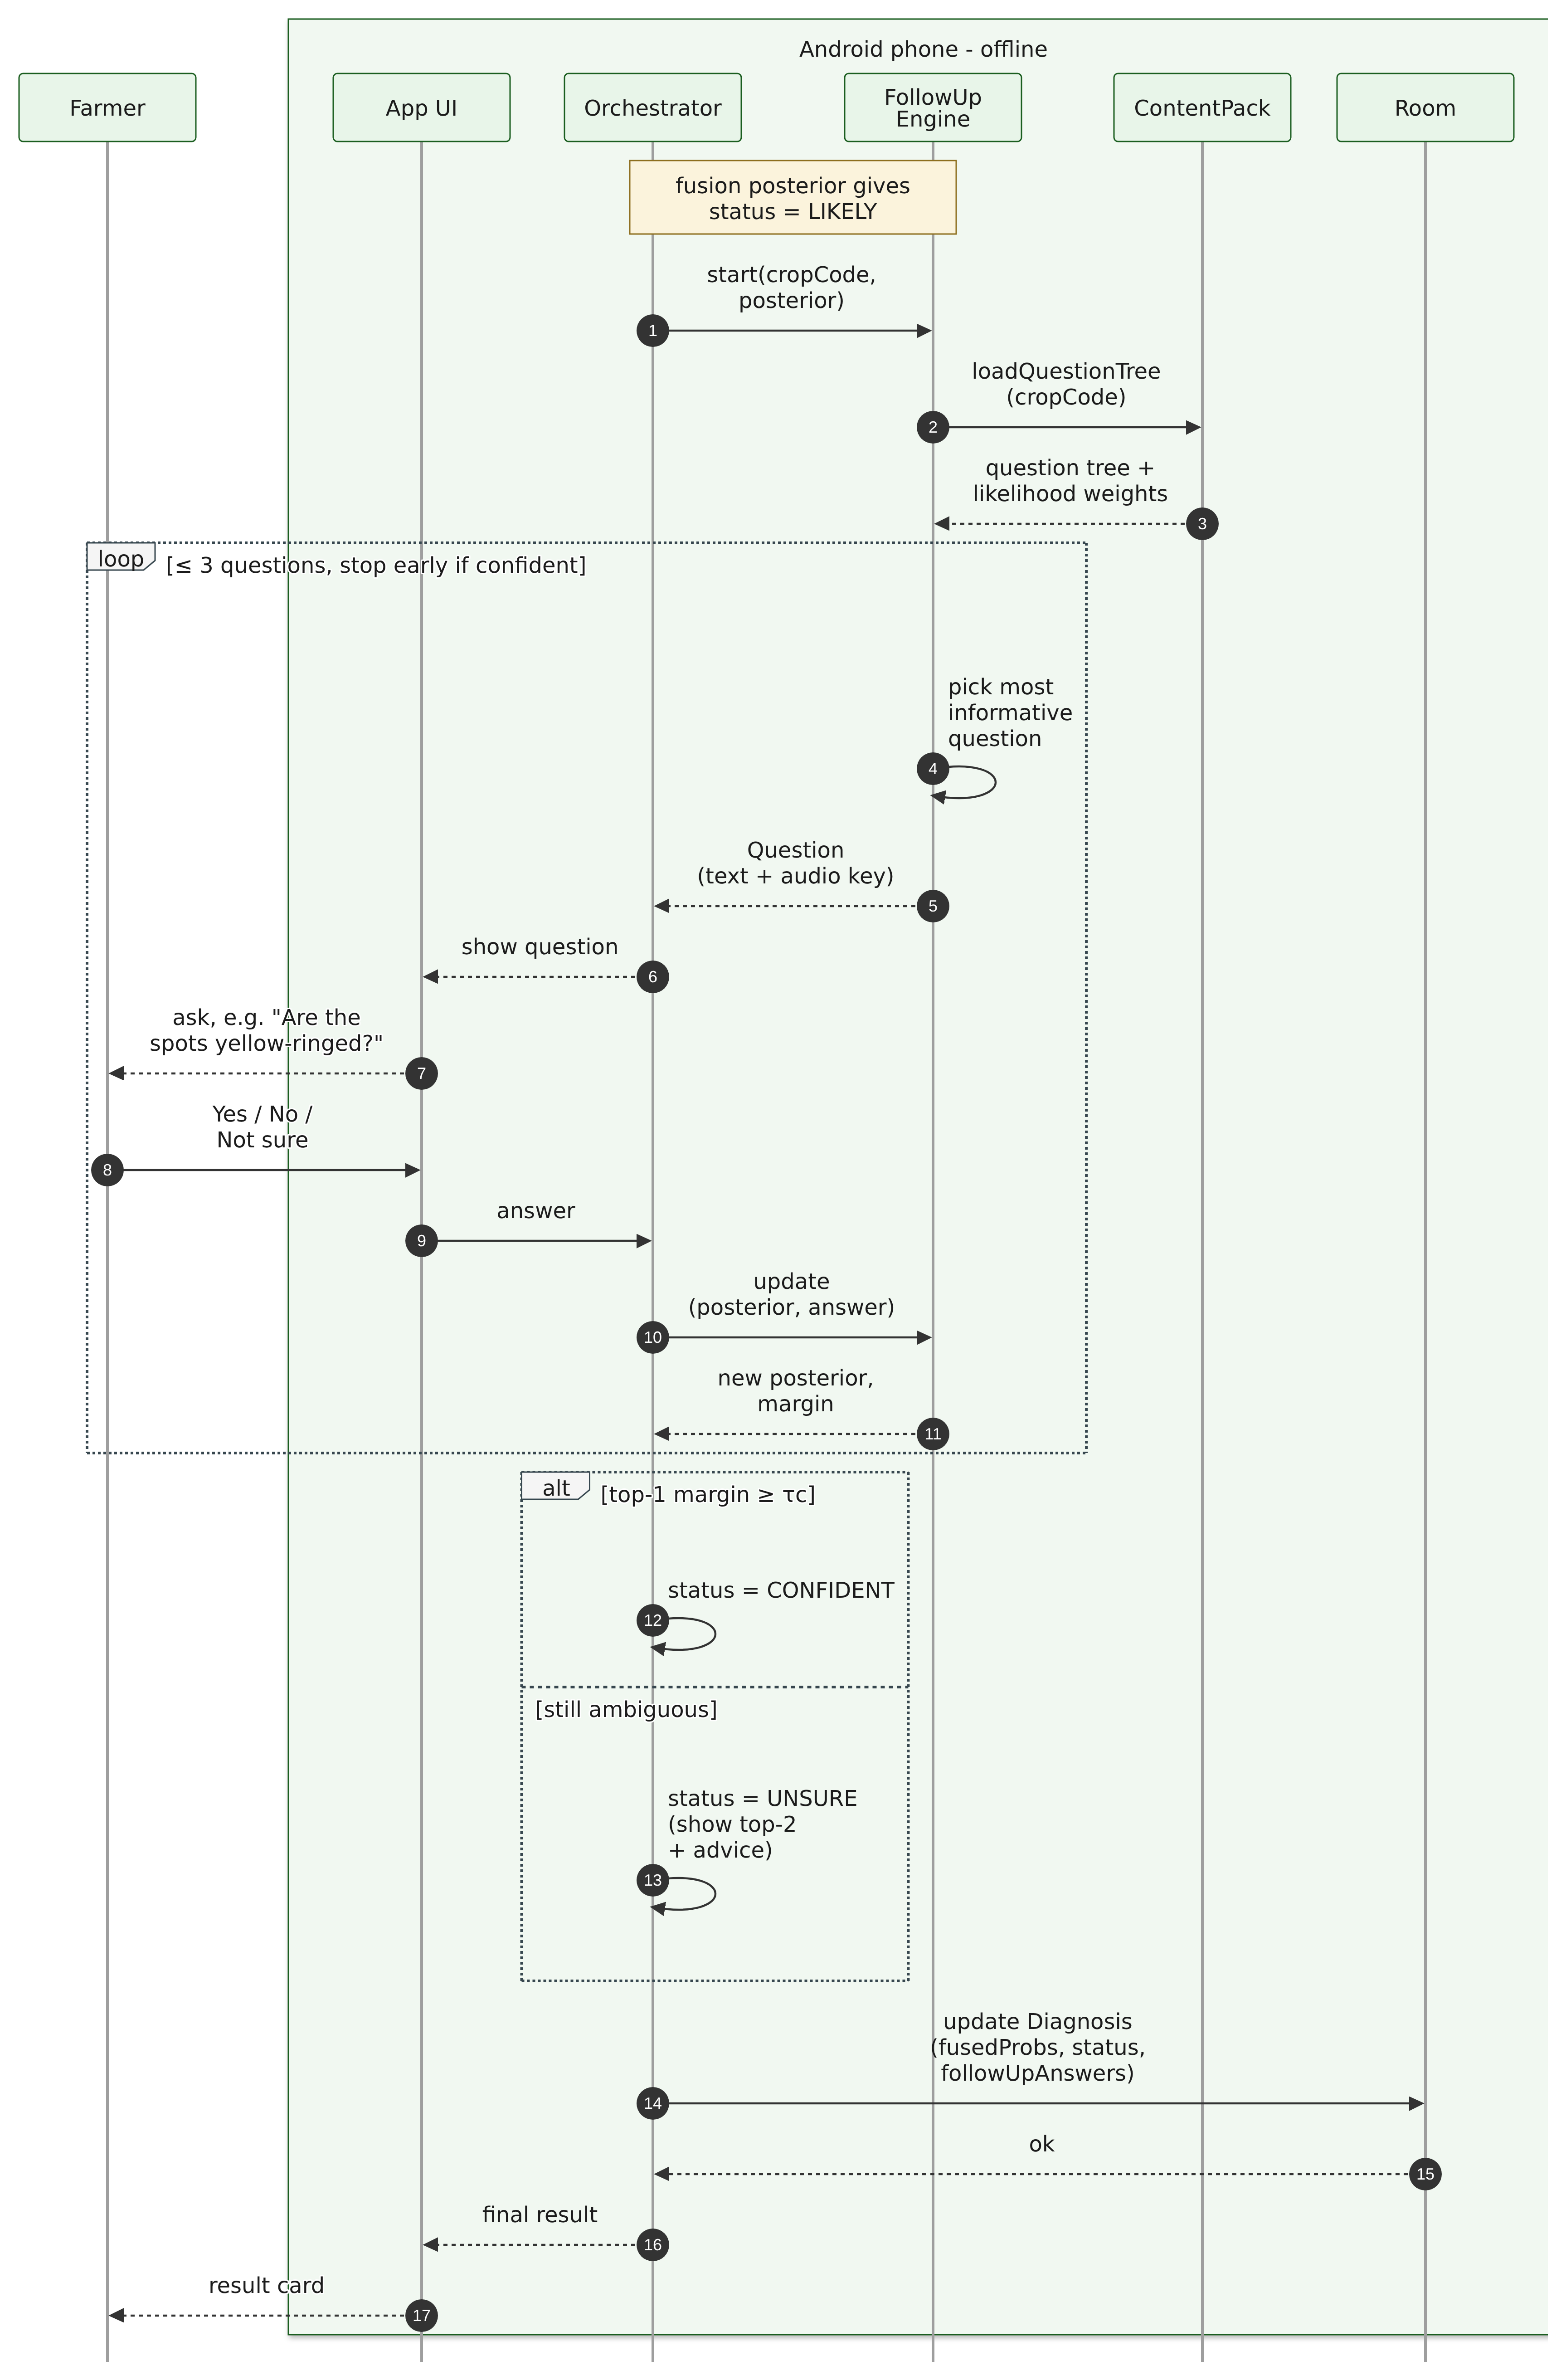
\includegraphics[width=\textwidth,height=0.88\textheight,keepaspectratio]{Figures/diagrams/seq_followup.png}
  \caption{Sequence diagram for the follow-up questions after a Likely outcome.}
  \label{fig:seq-follow}
\end{figure}

\textbf{Feedback synchronisation (UC-12, FR-24).} Figure~\ref{fig:seq-sync} shows feedback written locally as unsent, the background job that uploads it when connected, and the acknowledgement after which the local copy is deleted; offline, it simply stays queued.

\begin{figure}[H]
  \centering
  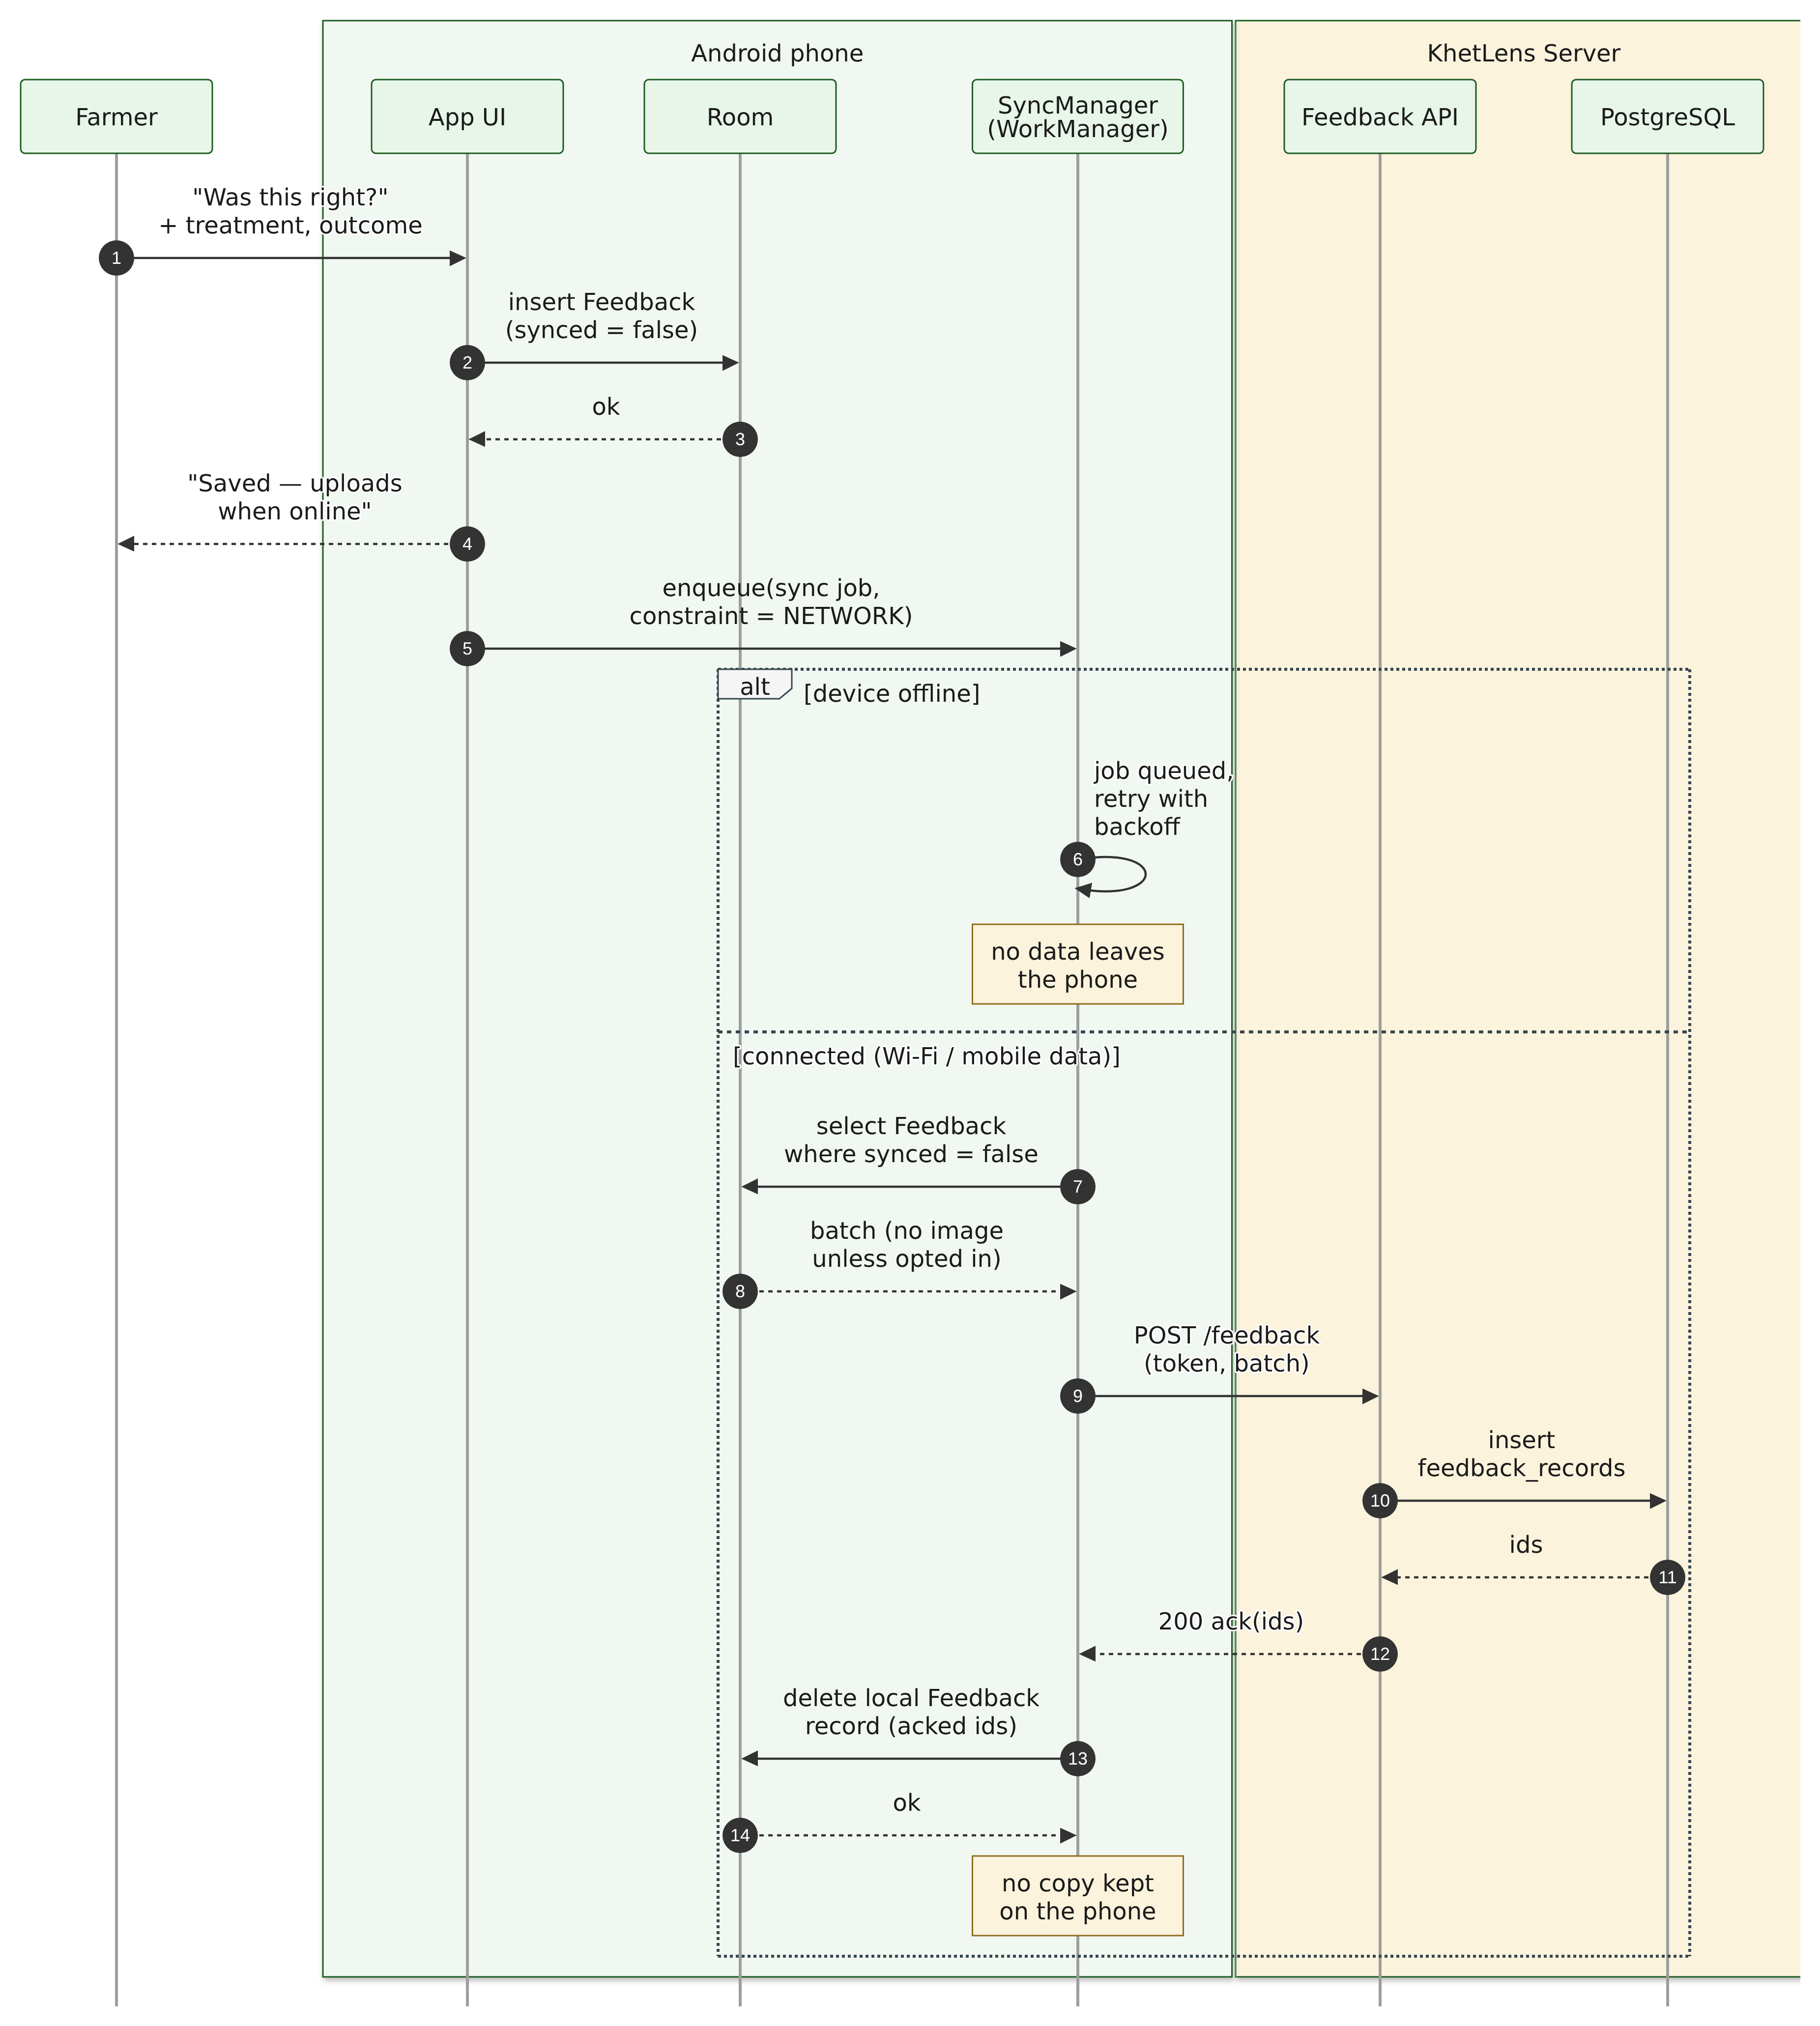
\includegraphics[width=\textwidth,height=0.88\textheight,keepaspectratio]{Figures/diagrams/seq_feedback_sync.png}
  \caption{Sequence diagram for offline feedback capture and later synchronisation.}
  \label{fig:seq-sync}
\end{figure}

\textbf{Sign-in (UC-02, UC-03).} Figure~\ref{fig:seq-login} shows the code request and verification through the server and the WhatsApp service, token storage, and the ``Skip for now'' alternative that creates a guest profile.

\begin{figure}[H]
  \centering
  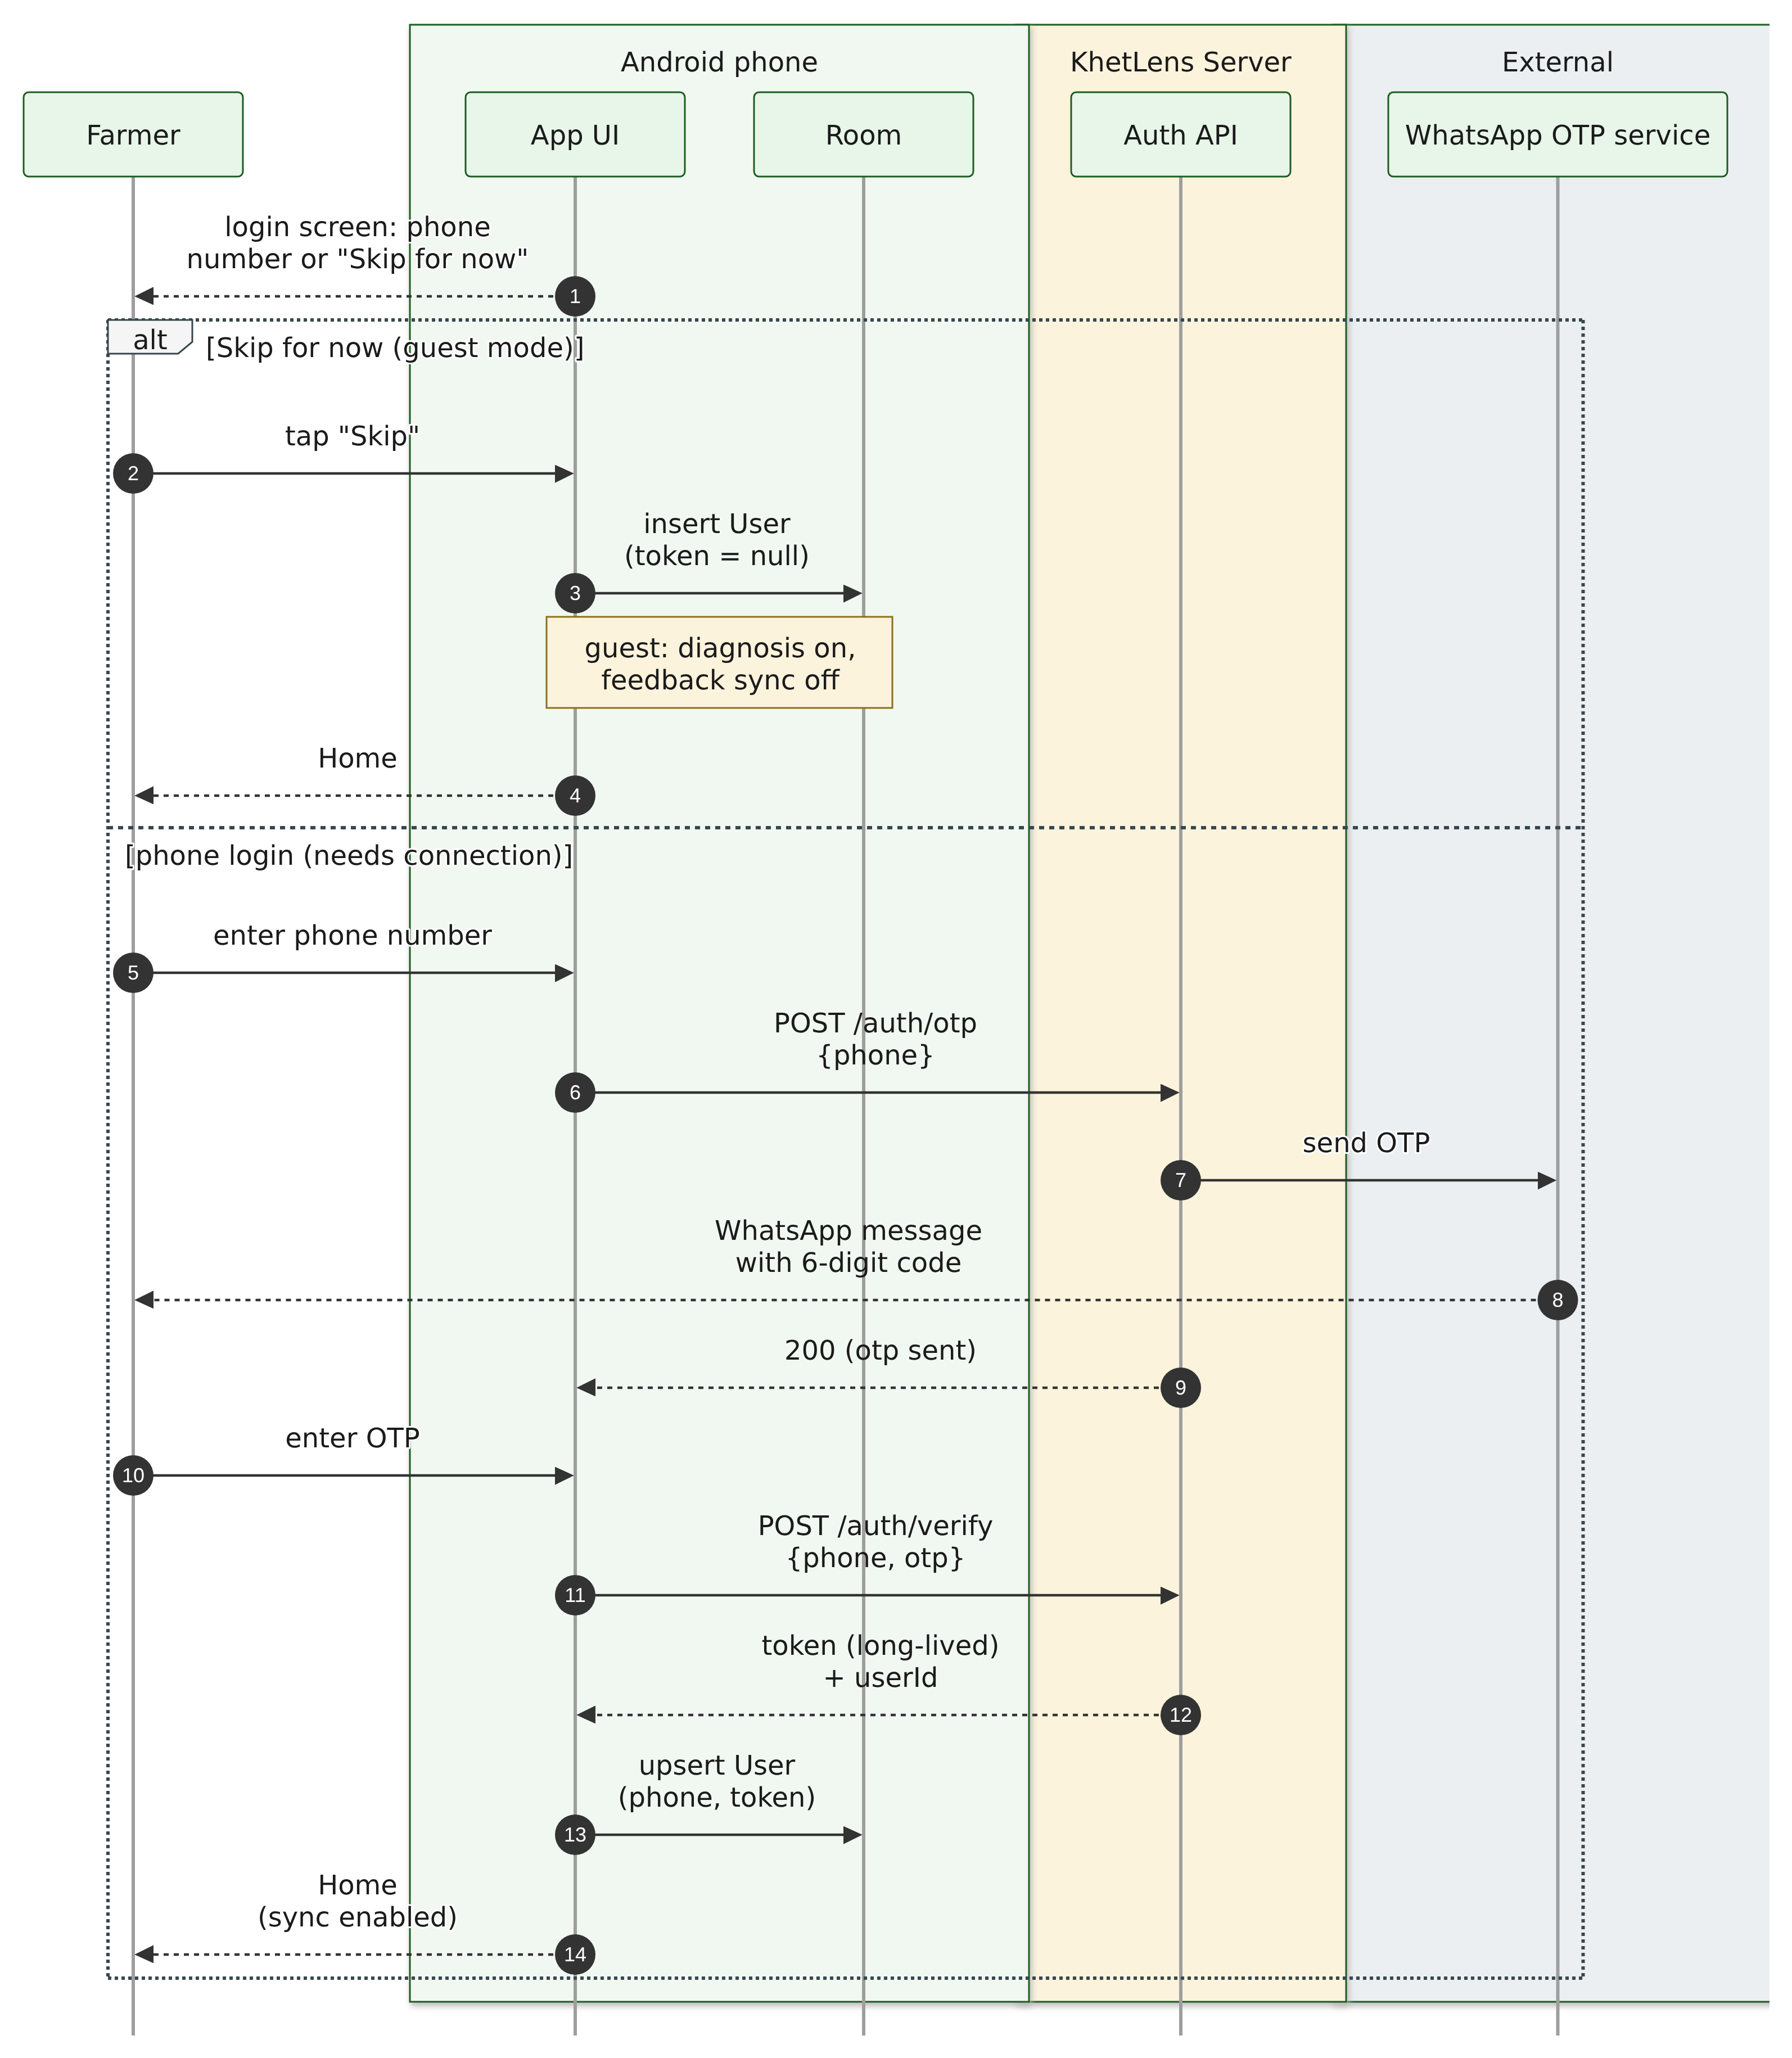
\includegraphics[width=\textwidth,height=0.88\textheight,keepaspectratio]{Figures/diagrams/seq_login.png}
  \caption{Sequence diagram for sign-in with a WhatsApp code and the guest-mode alternative.}
  \label{fig:seq-login}
\end{figure}

\textbf{Model and content update (UC-14).} Figure~\ref{fig:seq-update} shows the version check, background download, checksum verification, atomic switch and model reload, with the alternative that keeps the current version when the download fails.

\begin{figure}[H]
  \centering
  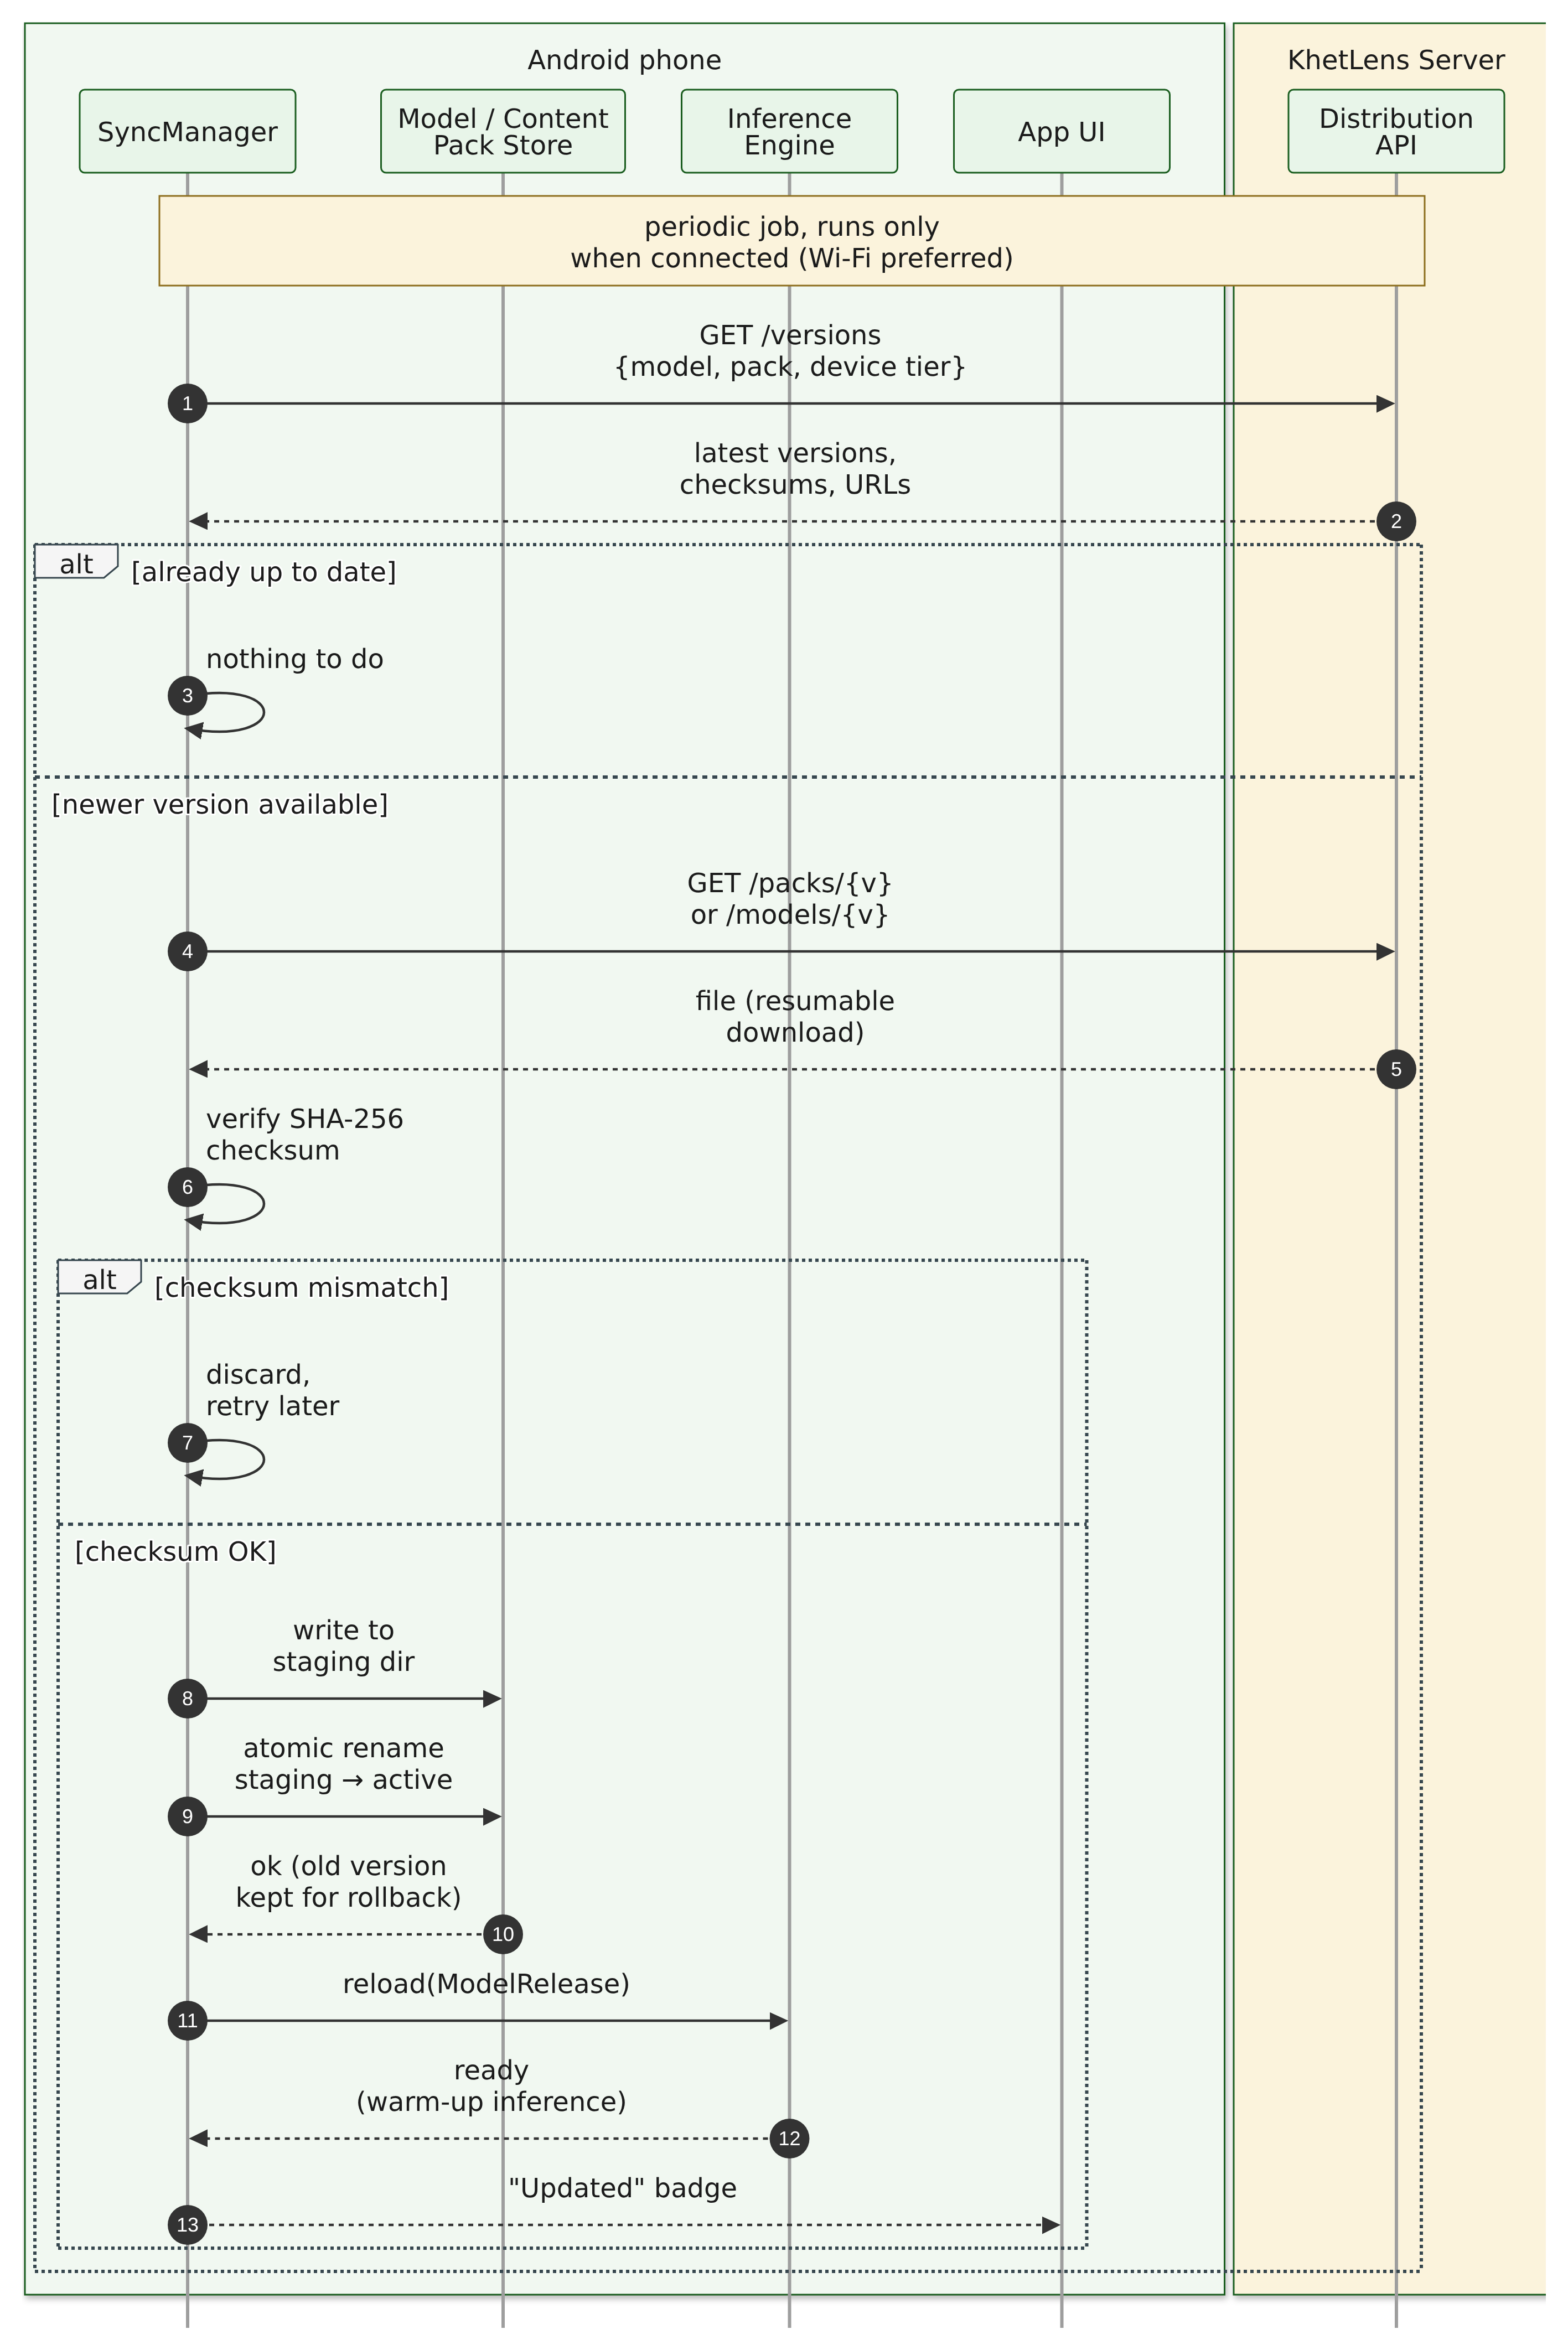
\includegraphics[width=\textwidth,height=0.88\textheight,keepaspectratio]{Figures/diagrams/seq_update.png}
  \caption{Sequence diagram for a model or content update.}
  \label{fig:seq-update}
\end{figure}

\section{Policies and Tactics}
\subsection{Conventions and coding guidelines}
Kotlin code follows the official Kotlin and Compose style guides, enforced by lint tools in the build; Python code follows PEP~8 with type hints. All user-visible strings live in resource files with Urdu and Punjabi translations. Requirement identifiers appear in test names and commit messages for traceability.

\subsection{Source layout and build}
The repository is a single project with \texttt{app/} (Android modules for presentation, domain, ML and data), \texttt{server/} (FastAPI), \texttt{training/} (data preparation, teacher, distillation, quantisation, export, calibration and the field-data study), \texttt{content/} (content sources, schema, audio) and \texttt{docs/}. A tagged release builds a signed APK and runs the test suite; model releases are produced by a single training script that runs export, calibration, contract tests and bundle creation; the publish tool uploads packs and releases to the server after validation. The APK ships with a bundled baseline model and content pack so that first launch works offline (FR-26).

\subsection{Choice of products}
TensorFlow Lite for inference (ONNX Runtime benchmarked); Room for persistence; WorkManager for background work; encrypted preferences for tokens; Noto Nastaliq Urdu and Noto Sans fonts; Opus audio; PostgreSQL; a free weather API behind a provider interface; a WhatsApp Business API provider for codes.

\subsection{Algorithms and idioms}
The diagnosis pipeline is a pure function of (image, weather, release parameters) with no hidden state, which makes it testable on the desktop with recorded inputs. Outcomes are a sealed type; repositories are interfaces; dependency injection wires the implementations.

\subsection{Requirements traceability and testing}
A traceability matrix (feature, functional requirements, use cases, design components, test cases) is kept with the documentation and will be presented in the implementation report. Unit tests cover the quality score, the thresholds, the fusion arithmetic, the question update and the repositories; contract tests load a model release and check tensor names, shapes and the manifest; instrumented tests run the farmer use cases with the network disabled; model acceptance tests compute NFR-04 and NFR-05 on the field test set for every release; farmer task tests are run with our partner's field officers.

\subsection{Maintenance and extensibility}
Adding a condition requires a new class in one disease head, a content entry and a weather-table row; adding a crop requires a new head and a new question set; changing the weather provider requires a new provider implementation. The model contract and content schema are versioned, and the app declines a release whose contract version it does not support.

\section{Conclusion}
This chapter has given the design that carries the methodology of Chapter~\ref{ch:method} to the farmer under the constraints of Chapter~\ref{ch:vision}: an offline-first native Android application with a four-layer architecture whose diagnostic core is a pure, testable function; a deliberately small backend; and an offline training pipeline whose releases are versioned artefacts consumed through a fixed contract. The architectural strategies record the alternatives we considered, the class and sequence diagrams specify the structure and behaviour at the level needed to begin implementation, and the policies define how the code will be written, tested, traced and maintained. Together with the requirements of Chapter~\ref{ch:srs}, this is the specification against which we will implement and test KhetLens.
